\documentclass{patmorin}
\listfiles
\usepackage{pat}
\usepackage{paralist}
\usepackage[OT1]{fontenc}
\usepackage[utf8]{inputenc}
\usepackage{paralist}
\usepackage{bbm}  % needed for \mathbbm{1}
% \usepackage{logix}
\usepackage{halloweenmath}
\usepackage{stmaryrd}

\usepackage{todonotes}
\usepackage{tcolorbox}

% etoolbox allows for robust commands that don't need \protect, e.g.
% \newrobustcmd{\onesub}{\mathord{\includegraphics{figs/one-sub}}}
% \subsection{Approximate Voronoi Diagrams in $G^{\onesub}_k$}
\usepackage{etoolbox}

% david proposes the following additions
\renewcommand{\ge}{\geqslant}
\renewcommand{\le}{\leqslant}
\renewcommand{\geq}{\geqslant}
\renewcommand{\leq}{\leqslant}

\newcommand{\david}[1]{{\color{orange} David: #1}}
\newcommand{\vida}[1]{{\color{DarkGreen} Vida: #1}}
\newcommand{\pat}[1]{\textcolor{Maroon}{Pat: #1}}
\newcommand{\gwen}[1]{\textcolor{Purple}{Gwen: #1}}
\newcommand{\piotr}[1]{\textcolor{red}{Piotr: #1}}


\newenvironment{clmproof}{\noindent\emph{Proof of Claim:}}{\hfill\rule{1ex}{1ex}}

\usepackage[longnamesfirst,numbers,sort&compress]{natbib}

\usepackage[mathlines]{lineno}
\setlength{\linenumbersep}{2em}
% \linenumbers
% \rightlinenumbers
% \linenumbers
\newcommand*\patchAmsMathEnvironmentForLineno[1]{%
 \expandafter\let\csname old#1\expandafter\endcsname\csname #1\endcsname
 \expandafter\let\csname oldend#1\expandafter\endcsname\csname end#1\endcsname
 \renewenvironment{#1}%
    {\linenomath\csname old#1\endcsname}%
    {\csname oldend#1\endcsname\endlinenomath}}%
\newcommand*\patchBothAmsMathEnvironmentsForLineno[1]{%
 \patchAmsMathEnvironmentForLineno{#1}%
 \patchAmsMathEnvironmentForLineno{#1*}}%
\AtBeginDocument{%
\patchBothAmsMathEnvironmentsForLineno{equation}%
\patchBothAmsMathEnvironmentsForLineno{align}%
\patchBothAmsMathEnvironmentsForLineno{flalign}%
\patchBothAmsMathEnvironmentsForLineno{alignat}%
\patchBothAmsMathEnvironmentsForLineno{gather}%
\patchBothAmsMathEnvironmentsForLineno{multline}%
}



% Taken from
% https://tex.stackexchange.com/questions/42726/align-but-show-one-equation-number-at-the-end
\newcommand\numberthis{\addtocounter{equation}{1}\tag{\theequation}}

\definecolor{brightmaroon}{rgb}{0.76, 0.13, 0.28}
\definecolor{linkblue}{rgb}{0, 0.337, 0.227}
\newcommand{\defin}[1]{\emph{\textcolor{brightmaroon}{#1}}}
\makeatletter
\def\mathcolor#1#{\@mathcolor{#1}}
\def\@mathcolor#1#2#3{%
  \protect\leavevmode
  \begingroup
    \color#1{#2}#3%
  \endgroup
}
\makeatother
\newcommand{\mathdefin}[1]{\mathcolor{brightmaroon}{#1}}
% \newcommand{\mathdefin}[1]{\color{brightmaroon}#1}}
\setlength{\parskip}{1ex}

% Document-specific commands and math operators
\DeclareMathOperator{\tw}{tw}
\DeclareMathOperator{\pw}{pw}
\DeclareMathOperator{\bw}{bw}
\DeclareMathOperator{\rtw}{rtw}
\DeclareMathOperator{\diam}{diam}
\DeclareMathOperator{\mindist}{min-dist}
\DeclareMathOperator{\ld}{ld}
\DeclareMathOperator{\polylog}{polylog}
\DeclareMathOperator{\evol}{Evol}
\DeclareMathOperator{\ivol}{Ivol}
\DeclareMathOperator{\tvol}{Tvol}


\title{\MakeUppercase{Fan-Partitions of Planar Graphs (and Beyond)
  \newline by Local Sparsification and Volume-Preserving Embeddings}}
\author{TBD}

% \author{
% Vida Dujmovi{\'c}\,\footnotemark[6]\qquad
% Gwena\"el Joret\,\footnotemark[4] \qquad
% Piotr Micek\,\footnotemark[5] \\
% Pat Morin\,\footnotemark[9]\qquad
% David~R.~Wood\,\footnotemark[2]
% }

% \footnotetext[2]{School of Mathematics, Monash University, Melbourne, Australia (\texttt{david.wood@monash.edu}). Research of Wood supported by the Australian Research Council.}

% \footnotetext[6]{School of Computer Science and Electrical Engineering, University of Ottawa, Ottawa, Canada (\texttt{vida.dujmovic@uottawa.ca}). Research supported by NSERC.}

% \footnotetext[4]{D\'epartement d'Informatique, Universit\'e libre de Bruxelles, Belgium (\texttt{\{gwenael.joret,michal.seweryn\}@ulb.be}). G.\ Joret is supported by a CDR grant from the Belgian National Fund for Scientific Research (FNRS), by a PDR grant from FNRS, and by the Australian Research Council.}

% \footnotetext[5]{Department of Theoretical Computer Science, Jagiellonian University, Kraków, Poland (\texttt{piotr.micek@uj.edu.pl}). Research supported
% the National Science Center of Poland under grant UMO-2018/31/G/ST1/03718 within the BEETHOVEN program.}

% \footnotetext[9]{School of Computer Science, Carleton University, Ottawa, Canada (\texttt{morin@scs.carleton.ca}). Research supported by NSERC and the Ontario Ministry of Research and Innovation.}


\date{}


\begin{document}

\maketitle

\begin{abstract}
  We show that every $n$-vertex planar graph is contained in the strong product of a fan and a clique of size $O(\sqrt{n}\log^2 n)$.  Equivalently, every $n$-vertex planar graph $G$ has a set $X$ of $O(\sqrt{n}\log^2 n)$ vertices such that $G-X$ has bandwidth $O(\sqrt{n}\log^2 n)$.  This result holds in the more general setting of product structured graphs, which includes bounded genus graphs and $k$-planar graphs for fixed $k$.
\end{abstract}

\section{Introduction}


The \defin{$k$-blowup} of a graph $H$ is the graph obtained by replacing each vertex $v$ of $H$ with a clique $K_v$ of size $k$ and replacing each edge $vw$ of $H$ with a complete bipartite graph with parts $V(K_v)$ and $V(K_w)$.  The current work is motivated by the following question: What is the simplest family of graphs $\mathcal{H}$ such that for each $n$-vertex planar graph $G$ there is a graph $H\in\mathcal{H}$ such that $G$ is contained in a $\tilde{O}(\sqrt{n})$-blowup of $H$, where $\tilde{O}$ notation hides $\polylog(n)$ terms?\footnote{We say that a graph $G$ is \defin{contained} in a graph $G'$ if $G$ is isomorphic to a subgraph of $G'$.}

\citet{ISW} show that one can take $\mathcal{H}$ to be the class of treewidth-$3$ graphs\footnote{A \defin{tree-decomposition} of a graph $G$ is a collection $(B_x)_{x \in V(T)}$ of subsets of $V(G)$ indexed by a tree $T$, such that: (a) for every edge ${vw \in E(G)}$, there exists a node ${x \in V(T)}$ with ${v,w \in B_x}$, and (b) for every vertex ${v \in V(G)}$, the set $\{ x \in V(T) \colon v \in B_x \}$ induces a non-empty (connected) subtree of $T$. The \defin{width} of such a tree-decomposition is ${\max\{ |B_x| \colon x \in V(T) \}-1}$. A \defin{path-decomposition} is a $P$-decomposition for any path $P$, denoted by the corresponding sequence of bags.
The \defin{treewidth $\tw(G)$} of a graph $G$ is the minimum width of a tree-decomposition of $G$.
The \defin{pathwidth $\pw(G)$} of a graph $G$ is the minimum width of a path-decomposition of $G$.
Treewidth is the standard measure of how similar a graph is to a tree.
Pathwidth is the standard measure of how similar a graph is to a path.}. \citet{distel.dujmovic.ea:product} show that the class of treewidth-$2$ graphs is sufficient.  In the current work, we show that one can even take $\mathcal{H}$ to be the class of fan graphs, which have pathwidth $2$.\footnote{A \defin{fan} $F_k$ is a graph with $V(F_k):=\{v_0,\ldots,v_k\}$ and $E(F_k):=\{v_0v_i:1\leq i\leq k\}\cup\{v_iv_{i+1}:1\leq i\leq k-1\}$. Note that $\{v_0,v_1,v_2\},\{v_0,v_2,v_3\},\dots,\{v_0,v_{k-1},v_k\}$ is a path-decomposition of $F_k$ with width 2.}

\begin{thm}\label{main_thm_planar}
  Every $n$-vertex planar graph is contained in a $O(\sqrt{n}\log^2 n)$-blowup of a fan.
\end{thm}

(We remark that the previous results \cite{ISW,distel.dujmovic.ea:product} have no polylogarithmic factors.  Every planar graphs is contained in a $O(\sqrt{n})$-blowup of a treewidth-$2$ graph \cite{distel.dujmovic.ea:product}.)

The choice of parameter $\sqrt{n}$ in these results is not arbitrary. A $k$-blowup of a treewidth-$t$ graph $H$ has treewidth at most $k(t+1)-1$.  Since there $n$-vertex planar graphs of treewidth $\Omega(\sqrt{n})$ (such as the $\sqrt{n}\times\sqrt{n}$ grid), any result like \cref{main_thm_planar} that finds all planar graphs in blowups of bounded treewidth graphs must have blowups of size $\Omega(\sqrt{n})$.  Pathwidth $2$ is also the best possible bound in theorems like  \cref{main_thm_planar}.  Indeed, even \emph{treewidth} $1$ is not achievable:  \citet{LMST08} describe an infinite family of $n$-vertex planar graphs $G$ such that every (improper) 2-colouring has a monochromatic component on $\Omega(n^{2/3})$ vertices. Say $G$ is contained in a $k$-blowup $(K_v:v\in V(T))$ of a tree $T$. Colour each vertex in each $K_v$ by the colour of $v$ in a proper 2-colouring of $T$. So each monochromatic component is contained in some $K_v$, implying that $k\in\Omega(n^{2/3})$.  \pat{The bound $O(n^{2/3})$ is achievable: Every $n$-vertex planar graph $G$ has a set $X$ of $O(n^{2/3})$ vertices such that every component of $G-X$ has size $O(n^{2/3})$ \cite{lipton.tarjan:applications}.  This implies that $G$ is an $O(n^{2/3})$-blowup of a star, where the set $X$ maps to the root of the star and each component of $G-X$ maps to a different leaf of the star.}
\pat{Mention that if $G$ is planar and has maximum degree $\Delta$ then $G$ is contained in the $O(\Delta\sqrt{n})$-blowup of a tree \cite{ding.oporowski:some}?}



\david{Stuff to add to the intro:
\begin{itemize}
\item $O(\sqrt{n})$ blowups of bounded treewidth graphs imply and strengthen the Lipton--Tarjan separator theorem. Without this, the naive reader will ask ``what is the point?''
\item \citet{distel.dujmovic.ea:product} asked whether every $n$-vertex planar graph is contained in a $O(\sqrt{n})$-blowup of a graph with bounded pathwidth. \cref{main_thm_planar} shows the answer is ``yes'' with $O(\sqrt{n})$ replaced by $\tilde{O}(\sqrt{n})$.
\item Results of \citet[Theorem~5]{DvoWoo} imply that for all $\epsilon>0$ there exists $c$ such that every $n$-vertex planar graph is contained in a $O(n^{1/2+\epsilon})$-blowup of a graph $H$ with treedepth $c$, which implies $\pw(H)\leq c-1$. \citet[Theorem~19]{DvoWoo} also establish a corresponding lower bound: for any $c\geq 1$ there exists $\epsilon>0$ such that if the $\sqrt{n}\times\sqrt{n}$ grid is contained in a $k$-blowup of a graph $H$ with treedepth at most $c$, then $k\geq\Omega(n^{1/2+\epsilon})$. (In fact, these lower and upper bounds match.)\ Thus the $\sqrt{n}\times \sqrt{n}$-grid is not contained in a $\tilde{O}(n^{1/2})$-blowup of a graph with bounded treedepth. In this sense, the `bounded pathwidth' condition in \cref{main_thm_planar} is best posible.
\item The fan in \cref{main_thm_planar} is of length $O(\sqrt{n}/\log^2 n)$. In general, if $\bw(G)\leq k$ then $G$ is contained in $P\boxtimes K_k$ where $|V(P)|=\ceil{|V(G)|/k}$. \pat{In \cref{bandwidth_relation}?}
\end{itemize}}


\subsection{Product Structured Graphs}

\cref{main_thm_planar} follows from a more general theorem about subgraphs of certain strong graph products, as we now explain.  The \defin{strong product} $A\boxtimes B$ of two graphs $A$ and $B$ is the graph with vertex set $V(A\boxtimes B):=V(A)\times V(B)$ that contains an edge with endpoints $(v_1,v_2)$ if and $(w_1,w_2)$ if and only if
\begin{compactenum}
    \item $v_1w_1\in E(A)$ and $v_2=w_2$;
    \item $v_1=w_1$ and $v_2w_2\in E(B)$; or
    \item $v_1w_1\in E(A)$ and $v_2w_2\in E(B)$.
\end{compactenum}
Note that $k$-blowup of $H$ can be written as the strong product $H\boxtimes K_k$.  Therefore, \cref{main_thm_planar} states that, for every $n$-vertex planar graph $G$ there is a fan $F$ such that $G$ is isomorphic to a subgraph of $F\boxtimes K_{O(\sqrt{n}\log^2 n)}$.

The \defin{row treewidth} of a graph $G$, denoted by $\rtw(G)$, is the minimum integer $t$ such that $G$ is contained in $H\boxtimes P$ for some graph $H$ with treewidth $t$ and for some path $P$. We prove the following more general result:

% Then \cref{main_thm_products} becomes: \\
% Every $n$-vertex graph with row-treewidth $t$ is contained in a $O(t\sqrt{n}\log^2 n)$-blowup of a fan.\\
% Much of the following discussion would be simplied.
% }

\begin{thm}\label{main_thm_products}
  Every $n$-vertex graph with row treewidth $t$ is contained in a $O(t\sqrt{n}\log^2 n)$-blowup of a fan.
\end{thm}

\Cref{main_thm_products} implies \cref{main_thm_planar} by the following \defin{Planar Graph Product Structure Theorem}:

\begin{thm}[\cite{dujmovic.joret.ea:planar,ueckerdt.wood.ea:improved}]\label{planar_product_structure}
  Every planar graph has row treewidth at most $6$.
\end{thm}

% \david{delete the following paragraph?} \Cref{planar_product_structure} has been generalized to a number of other minor-closed and non-minor closed graph classes (with $6$ replaced by some value that depends on the graph class), including bounded genus graphs and (more generally) apex-minor-free graphs \cite{dujmovic.joret.ea:planar,distel.hickingbotham.ea:improved} and $k$-planar graphs \cite{dujmovic.morin.ea:graph,distel.hickingbotham.ea:powers}.

\cref{main_thm_planar} generalises for graphs embeddable on arbitrary surfaces\footnote{The \defin{Euler genus} of a surface obtained from a sphere by adding $h$ handles and $c$ crosscaps is $2h+c$. The \defin{Euler genus} of a graph $G$ is the minimum Euler genus of a surface in which $G$ embeds without crossings.}.
Building on previous work in \citep{dujmovic.joret.ea:planar,ueckerdt.wood.ea:improved}, \citet{distel.hickingbotham.ea:improved} show that every graph of Euler genus $g$ has row treewidth at most $2g+6$. \Cref{main_thm_products} thus implies:

\begin{thm}\label{genus_products}
Every $n$-vertex graph of Euler genus $g$ is contained in a $O((g+1)\sqrt{n}\log^2 n)$-blowup of a fan.
\end{thm}

\pat{\Cref{genus_products} can be improved without using graph products. Every $n$-vertex genus-$g$ graph $G$ has a set of $X_0$ of $O(\sqrt{gn})$ vertices such that $G-X_0$ is planar \cite{eppstein:dynamic}. Apply \cref{main_thm_planar} to $G-X_0$ to get $X'$ of size $O(\sqrt{n}\log^2 n)$ such that $G-X_0-X'$ has bandwidth $O(\sqrt{n}\log^2 n)$.  Now take $X:=X_0\cup X'$ to get a set $X$ of size $O(\sqrt{gn} + \sqrt{n}\log^2 n)$ such that $G-X$ has bandwidth $O(\sqrt{n}\log^2 n)$.}

We have the following further generalisation\footnote{A graph $X$ is a \defin{minor} of a graph $G$ a graph isomorphic to $X$ can be obtained from a subgraph of $G$ by edge contractions. A graph $G$ is \defin{$X$-minor-free} if $X$ is not a minor of $G$.}.
A graph $X$ is \defin{apex} if $X-a$ is planar for some vertex $a\in V(X)$. \citet{dujmovic.joret.ea:planar} showed that for every apex graph $X$ there exists $c$ such that every $X$-minor-free graph has row treewidth at most $c$ (and such a theorem holds only if $X$ is apex). \cref{main_thm_products} thus implies:

\begin{thm}\label{apex_products}
For every fixed apex graph $X$, every $n$-vertex $X$-minor-free graph is contained in a $O(\sqrt{n}\log^2 n)$-blowup of a fan.
\end{thm}

Product structure theorems are known for various non-minor-closed classes~\citep{dujmovic.morin.ea:graph,HW24,distel.hickingbotham.ea:powers}. For example, a graph is \defin{$(g,k)$-planar} if it has a drawing in a surface of Euler genus $g$ with at most $k$ crossings on each edge. \citet{dujmovic.morin.ea:graph} proved that every $(g,k)$-planar graph has row treewidth  $O((g+1)k^5)$. \Cref{main_thm_products} thus implies:

\begin{thm}\label{gkplanar_products}
Every $n$-vertex $(g,k)$-planar graph is contained in a $O((g+1)k^5\sqrt{n}\log^2 n)$-blowup of a fan.
\end{thm}

\pat{Here's a better result, again without using product structure:  By the crossing lemma, $G$ has $O(\sqrt{k} n)$ edges (for $g\in O(n)$).  Add a dummy vertex at each crossing in $G$ to get a genus-$g$ graph $G'$ with $O(k^{3/2}(n+g))$ vertices.  Let $X_0'$ be a planarizing set of $G'$ of size $O(\sqrt{k^{3/2}(n+g)g})=O(k^{3/4}(\sqrt{n}+g))$ (again, using \citet{eppstein:dynamic}). Replace every dummy $x$ in $X_0'$ with (at most four) real vertices corresponding to the two edges that cross at $x$.  Now $G-X_0'$ is $k$-planar.  Add a dummy vertex at each crossing in $G-X_0'$ to get a planar graph $G''$ with $O(k^{3/2}n)$ vertices. Apply \cref{planar_sparsifier} to $G''$ to get $X''$ of size $O((k^{3/2}n/D)\log n)$ such that $G''$ has local density $D$.  By \cref{rao}, $G''$ has bandwidth $O(D\log^3 n)$.  Replace each dummy vertex in $X''$ by the (at most $4$) corresponding real vertices and let $X:=X_0'\cup X''$.  Then $|X|=O(k^{3/2}(\sqrt{n}+g)+(k^{3/2}n/D)\log n)$.  Take the $O(D\log^3 n)$-bandwidth ordering of $G''-X''$ and use it for the vertices of $G-X$.  Each edge of $G-X$ corresponds to a path of length at most $k+1$ in $G''-X''$, so this ordering has bandwidth $O(kD\log^3 n)$.  Set $D:=k^{1/4}\sqrt{n}/\log n$ to conclude that $G$ has fan-partition-width $O(g\sqrt{k} + k^{5/4}\sqrt{n}\log^2 n)$.\\[2ex]
It would be nice to shave off the ugly $k^{1/4}$ factor in this result.}

% \david{
% Do we get improved depedennce working with subgraph of $H\boxtimes P \boxtimes K_c$? (e.g. for $k$-planar graphs we can use $\tw(H)=10^{10}$ and $c=c_k$).
% }

% \pat{Now I can answer the question: No, the bound will be $O(tc\sqrt{n}\log^2 n)$.  The bottleneck is the sparsification lemma.  The size of the set $X$ there becomes $O((t+1)c(n/D)\log n)$.  Interestingly (maybe) when $G$ is a subgraph of $H\boxtimes P\boxtimes K_c$, the metric space $(V(G),d_{H\boxtimes P\boxtimes K_c})$ has $(k,O(t\sqrt{\log n}))$-volume-respecting embeddings, for any $c$. If you take $t=0$ and $c=n$ then you get a metric space where $d(v,w)=1$ for all  $v,w\in V(G)$ and this has as $(k,O(\sqrt{\log n}))$-volume respecting embedding.  The proof of this is much simpler: Every vertex maps to a uniformly random point in a $O(k\log n)$-dimensional ball of diameter $1$ (so the radius of the ball is $O(1/\sqrt{k\log n}))$.  Then the proof ``just'' boils down to showing that, with probability at least $1-n^{-ck}$, $k$ random points in this ball define a $(k-1)$-simplex whose $(k-1)$-dimensional volume is $\Omega((1/((k-1)!\sqrt{\log n})^{k-1}))$. \\[2ex]
% We should somehow get this point across in the introduction:  The metric space $(V(G),d_G)$ is awkward to work with directly for the same reason that planar graphs are awkward to work with directly; it's hard to see any structure.  The metric space $(V(G),d_{K_n})$ is a contraction of $(V(G),d_G)$ which makes it suitable to work with, and it's highly regular, but it's too ``dense'' to have any useful properties.  The metric space $(V(G),d_{H\boxtimes P})$ is a perfect middle-ground; it's highly regular (like $(V(G),d_{K_n}))$ but ``sparse'' enough to admit a local sparsification lemma \david{include this paragraph as is}.\\[2ex]
% It might be a useful exercise to find what properties of a metric space are sufficient to prove a local sparsification lemma.  Here's a first try:\\[2ex]
% Let $(S,d)$ be a finite metric space, let $L_0\subseteq S$, and for each $0\le a\le b$, let $L_{[a,b]}:=\{x\in S: a\le d(x,L_0)\le b\}$.  Now I'm stuck.  There is no obvious notion of a set $X\subseteq S$ that separates two subsets $A,B$ of $S$.
% }

\subsection{Relation to Bandwidth}
\label{bandwidth_relation}

An \defin{$H$-partition} of a graph $G$ is a partition $\mathcal{P}:=\{B_x: x\in V(H)\}$ of $V(G)$ whose parts are indexed by the vertices of $H$ such that, for each edge $vw$ of $G$, $v$ and $w$ are in the same part or there exists an edge $xy$ of $H$ such that $v\in B_x$ and $w\in B_y$.  The \defin{width} of $\mathcal{P}$ is the maximum size of any part.  It follows immediately from this definition that $G$ has an $H$-partition of width $w$ if and only if $G$ is contained in $H\boxtimes K_w$. When $H$ is a member of some class $\mathcal{H}$ of graphs, we call an $H$-partition of $G$ an \defin{$\mathcal{H}$-partition} of $G$.  For example, if $H$ is path, tree, or fan, then we call an $H$-partition a path-partition, a tree-partition, or a fan-partition, respectively.  The \defin{$\mathcal{H}$-partition-width}  of a graph $G$ is the minimum integer $w$ such that $G$ has an $\mathcal{H}$-partition of width $w$. Thus, \cref{main_thm_planar} states that every $n$-vertex planar graph has fan-partition-width $O(\sqrt{n}\log^2 n)$.

%\david{Hyphenate $\mathcal{H}$-partition-width, fan-partition, fan-partition-width, path-partition, path-partition-width throughout}

Let $G$ be a graph and let $v_1,\ldots,v_n$ be an ordering of $V(G)$.  Then $v_1,\ldots,v_n$ has \defin{bandwidth} $\mathdefin{\bw_G(v_1,\ldots,v_n)}:=\{\max\{|j-i|: v_iv_j\in E(G)\}$.  The \defin{bandwidth} of $G$ is $\mathdefin{\bw(G)}:=\min\{\bw_G(v_1,\ldots,v_n):\text{$v_1,\ldots,v_n$ is a ordering of $V(G)$}\}$. The bandwidth of a graph $G$ is closely related to the path-partition-width of $G$.  Indeed, if $\bw_G(v_1,\ldots,v_n)=w$, and $P:=x_1,\ldots,x_{\lceil n/w\rceil}$ is a path, then setting $B_{x_i}:=\{v_j: (i-1)w+1 \le j \le iw\}$ for each $i\in\{1,\ldots,\lceil n/w\rceil\}$ gives a path-partition $\{B_{x}:x\in V(P)\}$ of width $w$.  In the other direction, if $P:=x_1,\ldots,x_k$ is a path and  $\{B_x:x\in V(P)\}$ is a path-partition of width $w$ then any ordering $v_1,\ldots,v_n$ of $V(G)$ that places all vertices of $B_{x_i}$ before those in $B_{x_{i+1}}$ for each $i\in\{1,\ldots,k-1\}$ has $\bw_G(v_1,\ldots,v_n)\le 2w-1$.  Thus, \cref{main_thm_planar} is equivalent to saying that every $n$-vertex planar graph $G$ has a set $X$ of  $O(\sqrt{n}\log^2 n)$ vertices (the part $B_{x_0}$ in a fan-partition of $G$) such that $G-X$ has bandwidth $O(\sqrt{n}\log^2 n)$.


\subsection{Techniques}

For a graph $G$ and any two vertices $v,w\in V(G)$, define the \defin{(graph) distance} between $v$ and $w$, denoted $\mathdefin{d_G(v,w)}$, as the minimum number of edges in any path in $G$ with endpoints $v$ and $w$ or define $d_G(v,w):=\infty$ if $v$ and $w$ are in different components of $G$.  For any $r\ge 0$ and any $v\in V(G)$, let $B_G(v,r):=\{w\in V(G):d_G(v,w)\le r\}$ denote the radius-$r$ ball in $G$ with center $v$.
The \defin{local density} of a graph $G$ is $\mathdefin{\ld(G)}:=\max\{(|B(v,r)|-1)/r:r\ge 0,\, v\in V(G)\}$.\footnote{The ${}-1$ in this definition of local density does not appear in the definitions of local density used in some other works \cite{feige:approximating,rao:small}, but this makes no difference to our asymptotics results.  Our definition makes for cleaner formulas and seems to be more natural. For example, under our definition, the local density of a cycle of length $2k+1$ is $2$ and every $r$-ball contains exactly $2r-1$ vertices for $r\in\{1,\ldots,k\}$. Without the ${}-1$, the local density of a cycle is $3$, but only because radius-$1$ balls contain three vertices.} The local density of $G$ provides a lower bound on the bandwidth of $G$. For any ordering $v_1,\dots,v_n$ of $V(G)$ with bandwidth $b$, for each vertex $v_i$, $B_G(v_i,r) \subseteq \{v_{i-rb},\dots,v_{i+rb}\}$, so $|B_G(v_i,r)|\leq 2rb+1$ and $\ld(G)\leq 2\bw(G)$.
% } If $|B_G(v,r)|=Dr+1$ then in any permutation $v_1,\ldots,v_n$ of $V(G)$, one of the vertices $w$ in $B_G(v,r)\setminus \{v\}$ is at distance at least $Dr/2$ from $v$. That is, $v=v_i$ and $w=v_j$, and $|j-i|\ge Dr/2$.  Since $G$ contains a path with at most $r$ edges from $v$ to $w$, one of the edges $v_{i'}v_{j'}$ of this path must have $|i'-j'|\ge Dr/2r=D/2$.  Therefore $\bw(G)\ge\ld(G)/2$.
On the other hand, $\ld(G)$ is not upper bounded by any function of $\bw(G)$. In fact, \citet{CS89} describe a family of $n$-vertex trees $T$ with local density at most $9$, pathwidth $2$, and  $\bw(T)\in\Omega(\log n)$.
In his seminal work, \citet{feige:approximating} proves that bandwidth is also upper bounded by the local density and a polylogarithmic function of the number of vertices.

\begin{thm}[\citet{feige:approximating}]\label{feige_bandwidth_vs_density}
  For every $n$-vertex graph $G$,
  \[
    \bw(G)\in O\left(\ld(G)\cdot \log^3 n\sqrt{\log n\log\log n}\right) \enspace .
  \]
\end{thm}

\citet{rao:small} improves \cref{feige_bandwidth_vs_density} in the special case of planar graphs:%\footnote{\citet{rao:small} does not explicitly consider bandwidth, but his results on volume-preserving embeddings of planar graphs combined with the argument of \citet{feige:approximating} implies \cref{feige_bandwidth_vs_density}.}

\begin{thm}[\citet{rao:small}]
\label{rao_bandwidth_vs_density}
  For every $n$-vertex planar graph $G$,
  \[
    \bw(G)\in O\left(\ld(G)\cdot \log^3 n\right) \enspace .
  \]
\end{thm}

By \cref{rao_bandwidth_vs_density}, to prove \cref{main_thm_planar} it is sufficient to show the following \defin{local sparsification lemma}:

\begin{lem}\label{planar_sparsification_special}
  Every $n$-vertex planar graph $G$ has a set $X$ of $O(\sqrt{n}\log^2 n)$ vertices such that $\ld(G-X)\in O(\sqrt{n}/\log n)$.
\end{lem}

% For an example of \cref{planar_sparsification_special}, consider a complete binary tree $T_h$ of vertex height $h$.  Then $T_h$ has $n:=2^{h}-1$ vertices, and local density $(n-1)/(h-1)=\Theta(n/\log n)$. If we take $X$ to be the set of vertices in $T_h$ with vertex-depth $\lceil h/2\rceil$ then each component of $T_h-X$ has size $O(\sqrt{n})$ and local density $O(\sqrt{n}/\log n)$.

\Cref{planar_sparsifier}, in \cref{local_sparsification_section}, is a generalization of \cref{planar_sparsification_special} that trades off the size of $X$ against the local density of $G-X$.

Proving \cref{main_thm_products} takes somewhat more effort, for reasons that we now explain.
\Cref{rao_bandwidth_vs_density} is not stated explicitly in \cite{rao:small}. \citet{rao:small} shows that $n$-vertex planar graphs have $(k,O(\sqrt{\log n})$-volume-preserving Euclidean contractions (defined in \cref{contractions_section}). \citet{feige:approximating} proves a result that upper-bounds the bandwidth of an $n$-vertex graph $G$ that has local density $D$ and has a $(k,\eta)$-volume-preserving Euclidean contraction.  The upper bound on $\bw(G)$ is a function of $n$, $D$, $k$, and $\eta$.\footnote{The precise tradeoff between all these parameters is not stated explicitly in \cite{feige:approximating}, but can be uncovered from Feige's proof, which considers the case where $k=\log n$ and $\eta=\sqrt{\log n}\sqrt{\log n+ k\log k}$.}  A generalization of Feige's result is stated in \cref{volume_density_bandwidth}.  Combining these two results yields \cref{rao_bandwidth_vs_density}.

We follow a similar strategy.  We build a well-structured sparsifying set $X$ of size $O(\sqrt{n}\log^2 n)$ so that the metric space $(V(G),d_{(H\boxtimes P)-X)}$ has local density $D\in O(\sqrt{n}/\log n)$.  That is, any radius-$r$ ball in $(H\boxtimes P)-X$ contains at most $Dr-1$ vertices of $G$.  We then design a distance function $d^*$ that contracts the shortest path metric $d_{(H\boxtimes P)-X}$, in such a way that the metric space $(V(G),d^*)$ has local density $O(D)$ and also has a $(k,O(\sqrt{\log n})$-volume-preserving Euclidean contraction.  A generalization of Feige's result to metric spaces then establishes \cref{main_thm_products}.  A key element in our proof is that the distance function $d^*$ mixes distances measured in $H\boxtimes P$ with distance increases caused by large obstacles in $X$. This contracts the shortest path metric on $(H\boxtimes P)-X$ enough to prove the existence of a volume-preserving Euclidean contraction but not so much that it increases the local density.

% An important element of our proof is that we work in a metric space whose elements are vertices of $G$, but distances between vertices are measured in $H\boxtimes P$.  We do this for the same reason that the Product Structure Theorem (\cref{planar_product_structure}) has been so successful in resolving a number of longstanding problems on planar graphs \cite{dujmovic.joret.ea:planar,EJM23,DEJWW20,DEGJMM21}:  $H\boxtimes P$ is a supergraph of $G$ that still has many of the important properties of $G$ but its simple structure makes it easier to work with.  In our case, the graph $H\boxtimes P$ provides enough structure to prove a local sparsification lemma like \cref{planar_sparsification_special} even when local density is measured by counting the number of vertices of $G$ contained in balls of $(H\boxtimes P)-X$.  On the other hand, $H\boxtimes P$ is so well structured that, for a carefully chosen sparsifying set $X$, we can define a distance function $d^*$ over $V(G-X)$ for which we can modify Rao's techniques to bound the bandwidth of the metric space $(V(G-X),d^*)$. Despite being simple enough for this, $d^*$ captures enough detail about distances in $G-X$ that the bandwidth of the metric space $(V(G-X),d^*)$ effectively upper bounds the bandwidth of $G-X$.


\david{To illustrate \cref{planar_sparsification_special}, would it help to give the complete binary tree has an example? Here the bandwidth is at least $\frac{n}{\log n}$ (by local density). Deleting the middle layer of the tree, which has roughly $\sqrt{n}$ vertices, leaves a graph with bandwidth roughly $\frac{\sqrt{n}}{\log n}$. I expect this is necessary: I guess for any $m$ one needs to delete $m$ vertices to reduce the bandwidth to $n/( m\log(n/m))$. }

\pat{I started to do this, but then realized that, in this case, you get a components of size $O(\sqrt{n})$.  Unless we talk the optimal trade-off between separator size and component size, it might give the impression that we could ask for more:  A set $X$ of size $\tilde{O}(\sqrt{n})$ such that each component of $G-X$ has size $\tilde{O}(\sqrt{n})$.  }

\section{Background}

\subsection{Distance Functions and Metric Spaces}

A \defin{distance function} over a set $S$ is any function $d:S^2\to\R$ that satisfies $d(x,x)=0$ for all $x\in S$, $d(x,y)\ge 0$ and $d(x,y)=d(y,x)$ for all distinct $x,y\in S$, and $d(x,z) \le d(x,y)+d(y,z)$ for all distinct $x,y,z\in S$.  For any $x\in S$, $d(x,\emptyset):=\infty$ and, for any non-empty $Z\subseteq S$, $d(x,Z):=\min\{d(x,y):y\in Z\}$.  A \defin{metric space} $\mathcal{M}:=(S,d)$ consists of a set $S$ and a distance function $d$ over some superset of $S$. $\mathcal{M}$ is \defin{finite} if $S$ is finite and $\mathcal{M}$ is \defin{non-empty} is $S$ is non-empty.  For $x\in S$ and $r\geq 0$, the \defin{$r$-ball} centered at $x$ is $\mathdefin{B_{\mathcal{M}}(x,r)}:=\{y\in S:d(x,y)\le r\}$.  The \defin{diameter} of a non-empty finite metric space $(S,d)$ is $\mathdefin{\diam_d(S)}:=\max\{d(x,y):y\in S\}$, and the
\defin{minimum-distance} of $(S,d)$ is $\mathdefin{\mindist_d(S)}:=\min\{d(x,y): \{x,y\}\in\binom{S}{2}\}$.

For any graph $G$, $d_G$ is a distance function over $G$ and $\mathdefin{\mathcal{M}_G}:=(V(G),d_G)$ is a metric space. Any metric space that can be defined this way is referred to as a \defin{graph metric}. For any $S\subseteq V(G)$, the \defin{diameter} and \defin{minimum-distance} of $S$ in $G$ are defined as $\mathdefin{\diam_G(S)}:=\diam_{d_G}(S)$ and $\mathdefin{\mindist_G(S)}:=\mindist_{d_G}(S)$, respectively. In recent work on coarse graph theory~(e.g.~\citep{DN23,BBEGLPS}), $\diam_G(S)$ is called the `weak diameter' of $S$, to distinguish it from the diameter of $G[S]$.
% For $v\in V(G)$ and $W\subseteq V(G)$, $\mathdefin{d_G(v,W)}:=\min\{w\in W:d_G(v,w)\}$.
The \defin{positive distance in $G$} between $v\in V(G)$ and $W\subseteq V(G)$ is $\mathdefin{d^+_G(v,W)}:=\max\{1,d_G(v,W)\}$.
Since we will be working frequently with strong products. It is worth noting that, for any two graphs $A$ and $B$,
\[
  d_{A\boxtimes B}((x_1,x_2),(y_1,y_2))=\max\{d_A(x_1,y_1),d_B(x_2,y_2)\} \enspace .
\]

The \defin{local density} of a non-empty finite metric space $\mathcal{M}:=(S,d)$ is $$\mathdefin{\ld(\mathcal{M})}:=\max\{|(B_{\mathcal{M}}(x,r)-1)/r:x\in S,\, r>0\}.$$
\david{So that is is clear that this maximum exists, should we explain that since $S$ is finite there are only finitely many values of $r$ that need to be considered?}
Thus, if $\mathcal{M}$ has local density at most $D$ then $|B_{\mathcal{M}}(x,r)|\le Dr+1$ for each $x\in S$ and $r\ge 0$.
This definition is consistent with the definition of local density of graphs:  A connected graph $G$ has local density at most $D$ if and only if the metric space $\mathcal{M}_G$ has local density at most $D$.  Note that, if $(S,d)$ has local density at most $D$ then $(S,d)$ has $\diam_d(S)\ge (|S|-1)/D$ and $\mindist(S)\ge 1/D$.

A \defin{contraction} of a metric space $\mathcal{M}:=(S,d)$ into a metric space $\mathcal{M'}:=(S',d')$ is a function $\phi:S\to S'$ that satisfies $d'(\phi(x),\phi(y))\le d(x,y)$, for each $x,y\in S$. The \defin{distortion} of $\phi$ is $\max\{d(x,y)/d'(\phi(x),\phi(y)):\{x,y\}\in \binom{S}{2}\}$.\footnote{If there exists $x,y\in S$ with $d(x,y)>0$ and $d'(\phi(x),\phi(y))=0$ then the distortion of $\phi$ is undefined, or infinite. This will never be the case for any of the contractions we consider in this work.}  When $S\subseteq S'$ and $\phi$ is the identity function we say that $\mathcal{M'}$ is a contraction of $\mathcal{M}$. In particular, saying that $(S,d')$ is a contraction of $(S,d)$ is equivalent saying that $d'(x,y)\le d(x,y)$ for all $x,y\in S$.

For two points $x,y\in\R^L$, let $\mathdefin{d_2(x,y)}$ denote the Euclidean distance between $x$ and $y$.  A contraction of $(S,d)$ into $(\R^L, d_2)$ for some $L\ge 1$ is called a \defin{Euclidean contraction}.  For $K\subseteq S$ we abuse notation slightly with the shorthand $\mathdefin{\phi(K)}:=\{\phi(x):x\in K\}$.   We make use of two easy observations that follow quickly from these definitions:

\begin{obs}\label{contraction_increases_density}
  If a metric space $\mathcal{M}:=(S,d)$ has a contraction $\phi$ into a metric space $\mathcal{M}':=(S',d')$ of local density at most $D$, then $\mathcal{M}$ has local density at most $D$.
\end{obs}

\begin{proof}
  For any $x\in S$, any $r\ge 1$, and any $y\in B_\mathcal{M}(x,r)$, $d'(\phi(x),\phi(y))\le d(x,y)\le r$, since $\phi$ is a contraction.  Therefore, $B_{\mathcal{M'}}(\phi(x),r)\supseteq \phi(B_{\mathcal{M}}(x,r))$.  Since $\mathcal{M'}$ has local density at most $D$,  $Dr+1 \ge |B_\mathcal{M'}(\phi(x),r)|\ge |B_{\mathcal{M}}(x,r)|$.
\end{proof}

\begin{obs}\label{supergraph_contraction}
  For any connected graph $I$ and any connected subgraph $G$ of $I$, $(V(G),d_I)$ is a contraction of $(V(G),d_G)$.
\end{obs}

\begin{proof}
  From the definitions, it follows that $d_I$, restricted to $V(G)$ is a distance function over $V(G)$, so $(V(G),d_I)$ is a metric space.  Since $G$ is a subgraph of $I$, every path in $G$ is also a path in $I$ so, $d_I(x,y)\le d_G(x,y)$ for each $x,y\in V(G)$.  Therefore $(V(G),d_I)$ is a contraction of $(V(G),d_G)$.
\end{proof}

% \begin{obs}
%   If $\phi$ is a $(k,\eta)$-volume-preserving contraction of some metric space $\mathcal{M}$ and $\mathcal{M}$ is contraction of $\mathcal{M}'$
% \end{obs}


\subsection{Volume-Preserving Contractions}
\label{contractions_section}

For a set $K$ of $k\le L$ points in $\R^L$, the \defin{Euclidean volume} of $K$, denoted by $\mathdefin{\evol(K)}$, is the $(k-1)$-dimensional volume of the simplex whose vertices are the points in $K$.  For example, if $k=3$, then $\evol(K)$ is the area of the triangle whose vertices are $K$ and that is contained in a plane that contains $K$.

The \defin{ideal volume} of a finite metric space $(K,d)$ is defined as $$\mathdefin{\ivol_d(K)}:=\max\{\evol(\phi(K)):\text{$\phi$ is a Euclidean contraction of $(K,d)$}\}.$$  A Euclidean contraction $\phi:S\to\R^{\ell}$ of a finite metric space $(S,d)$ is \defin{$(k,\eta)$-volume-preserving} if $\evol(\phi(K))\ge \ivol_d(K)/\eta^{k-1}$ for each $k$-element subset $K$ of $S$.  This definition is a generalization of distortion: If $\phi$ is $(2,\eta)$-volume-preserving, then $\phi$ has dilation at most $\eta$.

\citet{feige:approximating} introduces the following definition and theorem as a bridge between ideal volume and Euclidean volume. The \defin{tree volume} of a finite metric space $(K,d)$ is defined as $\mathdefin{\tvol_d(K)}:=\prod_{xy\in E(T)} d(x,y)$ where $T$ is a minimum spanning tree of the weighted complete graph with vertex set $K$ where the weight of any edge $xy$ is equal to $d(x,y)$.  The following lemma make tree volume a useful intermediate measure when trying to establish that a contraction is volume-preserving.

\begin{lem}[{\citet[Theorem~3]{feige:approximating}}]
  Let $(S,d)$ be a finite metric space with $|S|=k$.  Then
  \[
    \ivol_{d}(S) \le \frac{\tvol_d(S)}{(k-1)!} \le 2^{(k-2)/2}\ivol_d(S) \enspace .
  \]
\end{lem}

\subsection{Bandwidth from Local Density and Volume-Preserving Contractions}

The following lemma generalizes \citet[Theorem~10]{feige:approximating} from graph metrics to general metric spaces and establishes a critical connection between local density and tree volume.

\begin{lem}[{\citet[Theorem~10]{feige:approximating}}]\label{reciprocal_sum}
  For any $n$-element metric space $\mathcal{M}:=(S,d)$ with local density at most $D$ and any positive integer $k$,
  \[
    \sum_{K\in \binom{V(G)}{k}}\frac{1}{\tvol_{d_G}(K)} < n(DH_n/2)^{k-1} \enspace ,
  \]
  where $\mathdefin{H_n}:=\sum_{i=1}^n 1/i\le 1+\ln n$ is the \defin{$n$-th harmonic number}.
\end{lem}

\begin{proof}
  First we claim that, for any $x\in S$,
  \begin{equation}
    \sum_{y\in S\setminus\{x\}} \frac{1}{d(x,y)} \le \sum_{i=1}^{n-1}\frac{1}{i/D} = DH_{n-1} < DH_n \enspace . \label{reciprocal_crux}
  \end{equation}
  To see why this is so, let $d_1\le\cdots\le d_{n-1}$ denote the distances of the elements in $S\setminus\{x\}$ from $x$.  For each $i\in\{1,\ldots,n-1\}$, let $\mathdefin{z_i}:=\max\{0\}\cup\{j: d_j \le i/D\}$. Observe that $z_i \le i$ since, otherwise $B_{(S,i/D)}(x,i/D)$ has radius $r:=i/D$ and size $j>i=rD$, contradicting the fact that $(S,d)$ has local density at most $D$.  If $z_i=i$ for each $i\in\{1,\ldots,n-1\}$ then $d_i=i/D$ for each $i\in\{1,\ldots,n-1\}$ and $\sum_{y\in S\setminus\{x\}}=\sum_{i=1}^{n-1}1/d_i=\sum_{i=1}^{n-1}\frac{1}{i/D}$, so \eqref{reciprocal_crux} holds.  Otherwise, consider the minimum $i$ such that $z_i < i$.  Then $z_i=i-1$, $d_{i-1}=(i-1)/D$ and $d_i > i/D$. By reducing $d_i$ to $i/D$ we increase $\sum_{i=1}^{n-1} 1/d_i$ and increase the minimum $i$ such that $z_i < i$.  Repeating this only increases $\sum_{i=1}^{n-1} 1/d_i$ and finishes with $\sum_{i=1}^{n-1} 1/d_i= H_{n-1}$.

  For a set $K$, let $\Pi(K)$ denote the set of all permutations $\pi:\{1,\ldots,k\}\to K$.
  \citet[Lemma~17]{feige:approximating} shows that, for any $k$-element subset $K$ of $S$,
  \[
    \frac{2^{k-1}}{\tvol(K)} \le \sum_{\pi\in\Pi(K)}\frac{1}{\prod_{i=1}^{k-1}d(\pi(i),\pi(i+1))}
  \]
  Therefore, to prove the lemma it is sufficient to show that
  \begin{equation}
    \sum_{K\in\binom{S}{k}}\sum_{\pi\in\Pi(K)}\frac{1}{\prod_{i=1}^{k-1}d(\pi(i),\pi(i+1))} \le n(DH_n)^{k-1} \enspace .
    \label{volume_sum}
  \end{equation}
  The proof is by induction on $k$.  When $k=1$, the outer sum in \cref{volume_sum} has $\binom{n}{1}=n$ terms, each inner sum has $1!=1$ terms, and the denominator in each term is an empty product whose value is $1$, by convention.  Therefore, for $k=1$, \cref{volume_sum} asserts that $n \le n$, which is certainly true.  Now assume that \cref{volume_sum} holds for $k-1$.  Then
  \begin{align*}
    & \quad \sum_{K\in\binom{S}{k}}\sum_{\pi\in\Pi(K)}\frac{1}{\prod_{i=1}^{k-1}d(\pi(i),\pi(i+1))} \\
    & = \sum_{K'\in\binom{S}{k-1}}\sum_{\pi\in\Pi(K')}\sum_{y\in S\setminus K'}\frac{1}{\prod_{i=1}^{k-2}d(\pi(i),\pi(i+1))}\cdot\frac{1}{d(\pi(k-1),y)} \\
    & = \sum_{K'\in\binom{S}{k-1}}\sum_{\pi\in\Pi(K')}\frac{1}{\prod_{i=1}^{k-2}d(\pi(i),\pi(i+1))}\cdot\sum_{y\in S\setminus K'}\frac{1}{d(\pi(k-1),y)} \\
    & \le \sum_{K'\in\binom{S}{k-1}}\sum_{\pi\in\Pi(K')}\frac{1}{\prod_{i=1}^{k-2}d(\pi(i),\pi(i+1))}\cdot DH_n & \text{(by \cref{reciprocal_crux})}\\
    & \le n(DH_n)^{k-2}DH_n & \text{(by induction)}\\
    & = n(DH_n)^{k-1} \enspace . & & \qedhere
  \end{align*}
\end{proof}

\Cref{volume_density_bandwidth}, below, is proved implicitly by \citet{feige:approximating} for graph metrics, although the dependence on the parameters $n$, $D$, $k$, and $\eta$ are not stated explicitly in \cite{feige:approximating}. Here we give a generalization for metric spaces and make the bound on the bandwidth explicit in terms of the parameters $n$, $D$, and $\eta$.

First, we need a definition of bandwidth for metric spaces.  Let $(S,d)$ be a finite metric space and let $x_1,\ldots,x_n$ be a permutation of $S$.  Then $\mathdefin{\bw_{(S,d)}(x_1,\ldots,x_n)}:=\max\{j-i:d(x_i,x_j)\le 1,\, 1\le i <j\le n\}$ and $\mathdefin{\bw(S,d)}$ is the minimum of $\bw_{(S,d)}(x_1,\ldots,x_n)$ taken over all $n!$ permutations $x_1,\ldots,x_n$ of $S$.  Note that this coincides with the definition of the bandwidth of a graph: For any connected graph $G$, $\bw(V(G),d_G)=\bw(G)$.  First we observe that injective
%\david{given that `injective' does not appear in the observation, why do we have `injective' here?} \pat{Laziness. In general, a contraction $\phi:A\to B$ of $(A,d_A)$ into $(B,d_B)$ need not be injective, in which case the observation isn't true.  If $B:=\{y\}$ and $\phi(x):=y$ for all $x\in A$ then $\bw(B,d_B)=0$, but this doesn't tell us anything about $\bw(A,d_A)$. The word injective is missing from the statement because saying that $(S,d')$ is a contraction of $(S,d)$ implicitly assumes that we are considering a contraction where $\phi$ is the identity function. I've added (injective) to the statement to remind the reader of this.}
contractions can only increase bandwidth:

%\david{given that `injective' does not appear in the observation, why do we have `injective' here?} \pat{Laziness. In general, a contraction $\phi:A\to B$ of $(A,d_A)$ into $(B,d_B)$ need not be injective, in which case the observation isn't true.  If $B:=\{y\}$ and $\phi(x):=y$ for all $x\in A$ then $\bw(B,d_B)=0$, but this doesn't tell us anything about $\bw(A,d_A)$. The word injective is missing from the statement because saying that $(S,d')$ is a contraction of $(S,d)$ implicitly assumes that we are considering a contraction where $\phi$ is the identity function. I've added (injective) to the statement to remind the reader of this.}

\begin{obs}\label{contraction_increases_bandwidth}
  For any finite metric space $\mathcal{M}:=(S,d)$ and any (injective) contraction $\mathcal{M}':=(S,d')$ of $\mathcal{M}$, $\bw(\mathcal{M}) \le \bw(\mathcal{M}')$.
\end{obs}

\begin{proof}
  Let $v_1,\ldots,v_n$ be an ordering of $S$ such that $b:=\bw(\mathcal{M}')=\bw_{\mathcal{M}}(v_1,\ldots,v_n)$. Consider any pair of vertices $v_iv_j$ with $d(v_i,v_j) \le 1$. Since $\mathcal{M}'$ is a contraction of $\mathcal{M}$, $d'(v_i,v_j)\le 1$.  Since $\bw_{\mathcal{M}'}(v_1,\ldots,v_n)\le b$, $|j-i|\le b$.  Thus $\bw(\mathcal{M})\le \bw_{\mathcal{M}}(v_1,\ldots,v_n)\le b$.
\end{proof}




\begin{thm}\label{volume_density_bandwidth}
  Let $(S,d)$ be a $n$-element metric space with local density at most $D$ and diameter at most $\Delta$.  If $(S,d)$ has a $(k,\eta)$-volume-respecting Euclidean contraction $\phi:S\to\R^L$
  % with $L\ge 4a\ln n$ --- not needed, I think
  then
  \[
    \bw(S,d) \in O((nk\log\Delta)^{1/k}\,Dk\eta\log^{3/2} n) \enspace .
  \]
\end{thm}

% \todo[inline]{Define a version of bandwidth for metric spaces. For a layout $x_1,\ldots,x_n$, $\bw(x_1,\ldots,x_n)=\max\{j-i:d(x_i,x_j)=1\}$. Because paths in graphs are made up of steps of length $1$, this is just the minimum distortion of a Euclidean embedding of $\phi:S\to\Z$.  I wonder if we could strengthen this theorem to show $(S,d)$ has an embedding where $|j-i|\le ?d(x_i,x_j)$?  Probably not!}

\begin{proof}
  Let $r$ be a random unit vector in $\R^L$ and for each $v\in S$, let $\mathdefin{h(v)}:=\langle r,\phi(v)\rangle$ be the inner product of $r$ and $\phi(v)$.  We will order the elements of $S$ as $v_1,\ldots,v_n$ so that $h(v_1)\le \cdots \le h(v_n)$.  To prove an upper bound on $\bw(S,d)$, it suffices to show an upper bound that holds with positive probability on the maximum, over all $vw$ with $d(v,w)\le 1$, of the number of vertices $x$ such that $h(v)\le h(x)\le h(w)$.

  Consider some pair $v,w\in S$ with $d(v,w)\le 1$. Since $\phi$ is a contraction, $d_2(\phi(v),\phi(w))\le 1$.  By \cite[Proposition~7]{feige:approximating}, $\Pr(|h(v)-h(w)|\ge \sqrt{4a\ln n/L}) \le n^{-a}$, for any $a\ge 1/4\ln n$. Therefore, with probability at least $1-n^{-a+2}$, $|h(v)-h(w)|\le \sqrt{4a\ln n/L}$ for each pair $v,w\in S$ with $d(v,w)\le 1$.

  Let  $K:=\{v_1,\ldots,v_k\}$ be a $k$-element subset of $S$. First observe that $\evol(\phi(K)\le n^k$, since $\evol(\phi(K))\le\prod_{i=2}^k d_2(\phi(v_{i-1}),\phi(v_i))\le \prod_{i=2}^k d(v_{i-1},v_i)\le \Delta^{k-2}$.  In particular, $\log\evol(\phi(K))\le k\log \Delta$.

  Define $\mathdefin{\ell(K)}:=\max_{v\in K}h(v)-\min_{v\in K} h(v)$.  By \cite[Theorem~9]{feige:approximating} there exists a universal constant $\beta$ such that, for any $c>0$,
  \[
      \Pr(\ell(K) \le c)
        < \frac{(\beta L)^{k/2}c^k\max\{1,\log(\evol(\phi(K))\}}{k^k\evol(\phi(K))}
        \le \frac{(\beta L)^{k/2}c^kk\log\Delta}{k^k\evol(\phi(K))} \enspace .
  \]
  In particular,
  \begin{align*}
    \Pr(\ell(K) \le \sqrt{4a\ln n/L})
      & <
      % \frac{(4\beta a\ln n)^{k/2}\max\{1,\log(\evol(\phi(K))\}}{k^k\evol(\phi(K))} \\
      % & <
      \frac{(4\beta a\ln n)^{k/2}\, k\log\Delta}{k^k\evol(\phi(K))} \\
      & \le \frac{(4\beta a\ln n)^{k/2}\eta^{k-1}\, k\log\Delta}{k^k\evol(\phi(K))} \\
      & \le \frac{(4\beta a\ln n)^{k/2}\eta^{k-1}(k-1)!2^{(k-2)/2}\, k\log\Delta}{k^k\tvol_{d}(K)} \\
      & \le \frac{(4\beta a\ln n)^{k/2}\eta^{k-1}2^{(k-2)/2}\,k\log\Delta}{\tvol_{d}(K)} \\
      & \le \frac{\left((8\beta a\ln n)^{1/2}\eta\right)^{k}\,k\log\Delta}{\tvol_{d}(K)} \\
  \end{align*}
  We say that $K\in\binom{S}{k}$ is \defin{bad} if $\ell(K) \le \sqrt{4a\ln n/L}$. Then the expected number of bad sets is at most
  \begin{align}
    \sum_{K\in \binom{S}{k}} \Pr(\text{$K$ is bad})
    & \le \sum_{K\in \binom{S}{k}} \frac{\left((8\beta a\ln n)^{1/2}\eta\right)^{k}\, k\log\Delta}{\tvol_{d}(K)} \notag \\
    & \le \left((8\beta a\ln n)^{1/2}\eta DH_n\right)^{k}\, nk\log\Delta
    & \text{(by \cref{reciprocal_sum})} \notag \\
    & \le \left(O(\eta D\log^{3/2}n)\right)^{k}\, nk\log\Delta \enspace .
    \label{bad_expectation}
  \end{align}
  Let $B$ a maximum cardinality subset of $S$ with $\ell(B)<\sqrt{4a\ln n/L}$.  The vertices in $B$ form $\binom{|B|}{k}$ bad sets. Therefore, by Markov's Inequality, the probability that $\binom{|B|}{k}$ exceeds \eqref{bad_expectation} by a factor of at least $2$ is at most $1/2$.  Therefore, with probability at least $1/2$, $\binom{|B|}{k}\le 2\cdot\eqref{bad_expectation}$, which implies that $|B|\in O((nk\log\Delta)^{1/k}\,Dk\eta\log^{3/2} n)$ with probability at least $1/2$.\footnote{Very roughly, $\binom{|B|}{k}$ is approximated by $(|B|/k)^k$.}  Therefore, with probability at least $1/2-n^{-a+2}$, $\bw_d(x_1,\ldots,x_n)\in O((nk\log\Delta)^{1/k}\,Dk\eta\log^{3/2} n)$.
\end{proof}


\section{Local Sparsification}
\label{local_sparsification_section}

In this section we will prove a generalization of the following result:

\begin{lem}\label{planar_sparsifier}
  For any $D\in\mathbb{R}$ with $1\leq D\leq n$, every $n$-vertex planar graph $G$ has a set $X$ of $O((n/D)\log n)$ vertices such that $G-X$ has local density at most $D$.
\end{lem}

Before continuing, we show that this, combined with the following result of \citet{rao:small}, establishes \cref{main_thm_planar}.

\begin{thm}[{\citet{rao:small}}]\label{rao}
  For every $k\le n$, every $n$-vertex planar graph $G$ has a $(k,O(\sqrt{\log n}))$-volume-preserving Euclidean contraction.
\end{thm}

Taking $k=\Theta(\log n)$ and combining \cref{rao,volume_density_bandwidth} yields the following corollary:

\begin{cor}\label{planar_density_bandwidth}
  Every $n$-vertex planar graph $G$ with local density at most $D$ has bandwidth $O(D\log^{3} n)$.
\end{cor}

% \begin{thm}\label{fan_partition_planar}
%   Every $n$-vertex planar graph $G$ contains a set $X$ of $O(\sqrt{n}\log^2 n)$ vertices such that $G-X$ has bandwidth $O(\sqrt{n}\log^2 n)$.
% \end{thm}

\begin{proof}[Proof of \cref{main_thm_planar}]
  Let $G$ be an $n$-vertex planar graph.  By \cref{planar_sparsifier}, $G$ contains a vertex set $X$ of size $O(\sqrt{n}\log^2 n)$ such that $G-X$ has local density at most $D:=\sqrt{n}/\log n$.  By \cref{planar_density_bandwidth}, $G-X$ has bandwidth at most $O(D\log^{3} n)=O(\sqrt{n}\log^2 n)$.
  % The theorem now follows from \cref{fan_partition_bandwidth}.
\end{proof}

% \pat{TODO: Insert the proof of \cref{planar_sparsifier} from David's WoGaG notes, which does the proof in Baker's setting: $G$ has a layering where any $\ell$ consecutive layers induces a subgraph of treewidth less than $(t+1)\ell$.  Later, we'll need to reuse the following lemma, which should be stated in terms of a weight function $w:V(H)\to\R_{\ge 0}$}.

% \begin{lem}\label{pq_separator}
% \david{I think $P$ and $D$ are poor notations, since they consistently mean something else earlier, and $D$ needs to be quantified. I would much rather state this result with an actual value for $c$ (e.g. $c=2$). From WoGaG Notes:  Fix $k\in\mathbb{N}$ and $p,q\in\mathbb{R}$ with $p\geq k$ and $q\geq 1$. Let $G$ be a graph with treewidth at most $k-1$. Fix $A\subseteq V(G)$  with $pq\geq k(|A|+1)$, which is implied if $pq\geq 2k|A|$. Then there exists a set $S$ of at most $p$ vertices in $G$ such that each component of $G-S$ has at most $q$ vertices in $A$. }
%   There exists a constant $c$ such that the following is true.
%   Let $G$ be an $n$-vertex graph of treewidth at most $t$ and let $P$ be a subset of $V(G)$.  Then \david{for any $D\in\mathbb{R}^+$?} there exists $X\subseteq V(G)$ of size at most $ct|P|/D$ such that each component of $G-X$ contains at most $D$ vertices in $P$.
% \end{lem}

The proof of \cref{planar_sparsifier} will make use of the following fairly standard vertex-weighted separator lemma.  Similar lemmas with similar proofs appear in  \citet{robertson.seymour:graph}, but we provide a proof for the sake of completeness.


\begin{lem}\label{weighted_separator}
    Let $H$ be a graph; let $\mathcal{T}:=(B_x:x\in V(T))$ be a tree decomposition of $H$; and let $\xi:V(H)\to\R$ be a function that is non-negative on $V(H)$.  For any subgraph $X$ of $T$, let       $\xi(X):=\sum_{v\in V(X)} \xi(v)$. Then, for any $c\in\N\setminus\{0\}$, there exists $S_T\subseteq V(T)$ of size $|S|\le c-1$ such that, for each component $X$ of $H-(\bigcup_{x\in S_T} B_x)$, $\xi(X)\le \xi(H)/c$.
\end{lem}

\begin{proof}
  The proof is by induction $c$.  The base case $c=1$ is trivial, since $S_T:=\emptyset$ satisfies the requirements of the lemma.  Now assume $c\ge 2$.  Root $T$ at some arbitrary vertex $r$ and for each $x\in V(T)$, let $T_x$ denote the subtree of $T$ induced by $x$ and all its descendants.  Let $H_x:=H[\bigcup_{y\in V(T_x)} B_y]$.  Say that a node $x$ of $T$ is \defin{heavy} if $\sum_{v\in V(H_x)} \xi(v) \ge \xi(H)/c$. Since $c\ge 1$, $r$ is heavy, so $T$ contains at least one heavy vertex. Let $x$ be a heavy vertex of $T$ with the property that no child of $x$ is also heavy.  Then $H':=H-V(H_x)$ has weight $\xi(H') = \xi(H)-\xi(H_x) \le (1-1/c)\cdot\xi(H)$.  On the other hand, every component $C$ of $H-V(H')-B_x$ has weight $\xi(C) \le \xi(H)/c$.  Apply induction on the graph $H'$ with tree decomposition $\mathcal{T}':=(B_x\cap V(H'):x\in V(T))$ and $c':=c-1$ to obtain a set $S'$ of size at most $c-2$ such that each component $X$ of $H'-(\bigcup_{x\in S} B_x)$, has weight $\xi(X) \le \tfrac{1}{c-1}\cdot(1-\tfrac{1}{c})\cdot\xi(H) = \tfrac{1}{c}\cdot \xi(H)$.  The set $S:=S'\cup\{x\}$ satisfies the requirements of the lemma.
\end{proof}

A \defin{layering} of a graph $G$ is a collection disjoint sets $\{L_s:s\in\Z\}$ indexed by integers whose union is $V(G)$ and such that, for each edge $vw$ of $G$, $v\in L_i$ and $w\in L_j$ implies that $|i-j|\le 1$.
A layering $\{L_s:s\in\Z\}$ has the \defin{$t$-Baker property} if, for every $s\in\Z$ and $r\in\N$, $G[L_s\cup\cdots\cup L_{s+r-1}]$ has treewidth at most $s(t+1)-1$. A graph $G$ has the \defin{$t$-Baker property} if $G$ has some layering with the $t$-Baker property.  Clearly if every connected compoonent of $G$ has the $t$-Baker property then $G$ has the $t$-Baker property.

It is a well known that planar graphs have the $2$-Baker property \cite{baker:approximation} and, for a connected planar graph $G$, any BFS layering of $G$ has the $2$-Baker property. Thus, \cref{planar_sparsifier} is an immediate consequence of the following result:

\begin{lem}\label{sparsifier_baker}
  Let $G$ be an $n$-vertex graph with the $t$-Baker property.  Then, for any $D\in\R$ with $1\le D\le n$, $G$ contains a set $X$ of at most $(18tn/D)\log n$ vertices such that $G-X$ has local density at most $D$.
\end{lem}

\begin{proof}
  Let $\{L_s:s\in Z\}$ be a layering of $G$ with the $t$-Baker property. For each positive integer $i$ and each integer $j$, let $G_{i,j}:=G[\bigcup_{s=j2^i}^{(j+1)2^i-1} L_s]$,  and let $G^+_{i,j}=G[V(G_{i,j-1})\cup V(G_{i,j})\cup V(G_{i,j+1})]$.  Observe that, for any $i$, the graphs in $\{ G_{i,j}\}_{j\in\N}$ are pairwise vertex disjoint.  By the definition $G^+_{i,j}$, this implies that the graphs in $\{ G_{i,j}\}_{j\in\N}$ have a total of at most $3n$ vertices.

  For each $i\in\{0,\ldots,\lfloor \log h\rfloor\}$ and each $j$, $G^+_{i,j}$ has treewidth at most $3t\cdot 2^i-1$.  By \cref{weighted_separator}, with weight function $\zeta(v):=1$ and $c=\lceil |V(G^+_{i,j})|/(D2^{i-1})\rceil$, there exists a set $X_{i,j}$ of size
  \[
    |X_{i,j}|\le 3t\cdot 2^i\cdot(c-1) =
    3t\cdot 2^i\cdot\left(\left\lceil\frac{ |V(G^+_{i,j})|}{D2^{i-1}}\right\rceil-1\right) \le
    \frac{3t\cdot 2^i\cdot|V(G^+_{i,j})|}{ D2^{i-1}}
    = \frac{6t|V(G^+_{i,j})|}{D}
  \]
  such that each component of $G^+_{i,j}-X_{i,j}$ has at most $|V(G^+_{i,j})|/c \le D2^{i-1}$ vertices.  Let $X:=\bigcup_{i=0}^{\lfloor\log h\rfloor-1}\bigcup_{j}X_{i,j}$.  Then
  \[
    |X| \le
    \sum_{i=0}^{\lfloor\log h\rfloor-1}\sum_{j} |X_{i,j}|
    \le
    \sum_{i=0}^{\lfloor\log h\rfloor-1}\sum_{j} \frac{6t|V(G^+_{i,j})|}{D}
    \le
    \sum_{i=0}^{\lfloor\log h\rfloor-1}\frac{18tn}{D}
    % \le
    % \frac{3(?3+1)n(1+\log h)}{D}
    % = O((n/D)\log n)
    \le \frac{18tn\log h}{D}\le\frac{18tn\log n}{D}
    \enspace .
    % \frac{3(?3+1)n(1+\log n)}{D}
  \]
  Now, consider some ball $B_{G-X}(v,r)$, let $i=\lceil\log r\rceil$, and let $j$ be the unique integer such that $v\in V(G_{i,j})$.  Then $B_{G-X}(v,r)$ is contained in a single component of $G^+_{i,j}-X_{i,j}$, and this component has at most $D2^{i-1}=D2^{\lceil\log r\rceil-1}\le Dr$ vertices.
\end{proof}




% \begin{proof}[Proof of \cref{planar_sparsifier} assuming \cref{sparsifier_simple}]
%   \citet{ueckerdt.wood.ea:improved} show that, for any planar graph $G$, there exists a graph $H$ of treewidth at most $6$ and a path $P$ such that $G$ is isomorphic to a subgraph of $H\boxtimes P$.  Without loss of generality, we treat $G$ as a subgraph of $H\boxtimes P$.  Apply \cref{sparsifier_simple} to $G$, $H$, and $P$ to obtain a set $X'\subseteq V(H\boxtimes P)$ of size $O((n/D)\log_2 n)$ and let $X:=V(G)\cap X'$.  Then $G-X$ is a subgraph of $H\boxtimes P-X'$ so, by \cref{supergraph_contraction}, $(V(G-X),d_{H\boxtimes P-X'})$ is a contraction of $(V(G-X),d_{G-X})$.  By \cref{contraction_increases_density}, the local density of $(V(G-X),d_{G-X})$ is at most the local density of $(V(G-X),d_{H\boxtimes P-X'})$, which is at most $D$.
% \end{proof}

% \Cref{sparsifier_simple} is a consequence of the following stronger technical lemma, which says that after removing the vertices in $X$, each component of the subgraph induced by $\ell$ consecutive layers of $H\boxtimes P-X$ contains at most $D\ell$ vertices of $G$.
% This immediately implies \cref{sparsifier_simple} because, for any vertex $v$ of $H\boxtimes P-X$ and any radius $r$,  $B_{H\boxtimes P-X}(v,r)$ is contained in at most $2r+1$ consecutive layers of $H\boxtimes P$, so $B_{H\boxtimes P-X}(v,r)$ contains at most $D(2r+1)\le 3Dr$ vertices of $G$.

% \begin{lem}\label{sparsifier}
%   For any graph $H$ of treewidth less than $t$, any path $P$, and any $n$-vertex subgraph $G$ of $H\boxtimes P$ there exists $X\subseteq V(H\boxtimes P)$ with $|X|\le ?t(n/D)\log_2 n$ such that each positive integer $\ell$, each $\ell$-vertex subpath $P'$ of $P$, and each component $C$ of $(H\boxtimes P)[V(H)\times V(P')]-X$ satisfies $|V(C)\cap V(G)|\le D\ell$.
% \end{lem}

% \begin{proof}[Proof of \cref{sparsifier_simple} assuming \cref{sparsifier}]
%   For any $v\in V(G)$, there exists a subpath $y_1,\ldots,y_{\ell}$ of $P$ with $\ell\le 2r+1$ such that $B_{H\boxtimes P}(v,r)$ is contained in $(H\boxtimes P)[V(H)\times \{y_1,\ldots,y_{\ell}\}]$.  Apply \cref{sparsifier} to $G$, $H$, $P$ and $D'=D/3$.  Then, for any $v$ and $r$, $B_{(H\boxtimes P)-X}(v,r)$ is contained in a single component $C$ of $(H\boxtimes P)[V(H)\times \{y_1,\ldots,y_{\ell}\}]-X$.  Thus $|V(C)\cap V(G)|\le D'\ell= D'(2r+1)\le 3D'r=D$.
% \end{proof}


% To prove \cref{sparsifier} we make use of the following frequently-used separator result (see, for example, \cite[Lemma~11]{bose.dujmovic.ea:asymptotically}):
%


\section{\boldmath Volume Preserving Embeddings of Subgraphs of $H\boxtimes P$}

% Let $G$ be a finite graph and let $\mathcal{D}:2^{V(G)}\to[0,1]$ be a probability distribution over subsets of $V(G)$.  Then $\mathcal{D}$ has the \defin{KPR$(\epsilon,\delta,\Delta)$-property} if
% \begin{compactenum}[(i)]
%   \item For each $Z$ in the support of $\mathcal{D}$, each component $C$ of $G-Z$ has $\diam_G(C)< \Delta$.
%   \item For each vertex $v$ of $G$ if we draw $Z$ according to the distribution $\mathcal{D}$, then
%   \[  \Pr(\text{$Z=\emptyset$ or $d_G(v,Z) \ge \floor{\epsilon\Delta})$})\ge \delta \enspace .
%   \]
% \end{compactenum}
% A graph $G$ has the \defin{KPR($\epsilon,\delta)$ property} if, for every positive integer $\Delta$, there exists a distribution $\mathcal{D}_\Delta$ over subsets of $V(G)$ that has the KPR$(\epsilon,\delta,\Delta)$-property.  A family $\mathcal{G}$ of graphs has the \defin{KPR property} if there exists some $\epsilon,\delta>0$ such that every graph in $\mathcal{G}$ has the KPR$(\epsilon,\delta)$ property.
%
% Building on the decomposition of \citet{klein.plotkin.ea:excluded}, \citet{rao:small} shows that planar graphs have the KPR property.  More generally,
%
% \begin{thm}
%   Every $K_{h}$-minor-free graph has the   KPH(\Omega,)
% \end{thm}
%


In this section, we prove \cref{main_thm_products}.  The structure of our proof is based on the proof of \cref{rao} by \citet{rao:small}, which applies to planar graphs and even to $K_{h}$-minor-free graphs for any fixed $h$.  However, the proof cannot be applied directly since graph products of the form $H\boxtimes P$ are not $K_h$-minor-free for any fixed $h$, even when $H$ is a tree and $P$ is a path. Indeed, if $T$ is the tree obtained from the path $P_{2n+1}$ by adding one leaf adjacent to the middle vertex, then $K_n$ is a minor of the `tennis court' graph $T\mathbin{\square} P_{n^2}$ (see  \citep{Wood-NYJM11}).

For the remainder of the paper, $G$ is an $n$-vertex subgraph of $H\boxtimes P$ where $H$ is a graph of treewidth $t$ and $P$ is a path.  The proof of \cref{main_thm_products} has the following structure. We use the notation $\mathcal{M}\rightbroom\mathcal{M'}$ to denote that $\mathcal{M}'$ is a contraction of $\mathcal{M}$.

\begin{enumerate}
  \item Use \cref{sparsifier_baker} to find a set $X\subseteq H\boxtimes P$ of size $O(\sqrt{n}\log^2 n)$ such that the metric space $\mathcal{M}:=(V(G-X),d_{(H\boxtimes P)-X})$ has local density $D\in O(\sqrt{n}/\log n)$.  Since $G-X$ is a subgraph of $(H\boxtimes P)-X$, $\mathcal{M}$ is a contraction of the metric space $\mathcal{M}_{G-X}:=(V(G-X),d_{G-x})$ (by \cref{supergraph_contraction}), so $\mathcal{M}_{G-X}\rightbroom\mathcal{M}$.

  \item Design a distance function $d^*:V((H\boxtimes P)-X)^2\to\R$ so that the metric space $\mathcal{M}^*:=(V(H\boxtimes P)\setminus X,d^*)$ is a contraction of $\mathcal{M}$ with the property that the induced metric space $(V(G-X),d^*)$ has local density $O(D)$.

  Graphically, $\mathcal{M}_{G-X}\rightbroom\mathcal{M}\rightbroom\mathcal{M}^*$.

  \item Prove that $\mathcal{M}^*$ has a $(k,O(\sqrt{\log n}))$-volume-preserving Euclidean contraction $\phi:V(H\boxtimes P)\setminus X\to\R^L$, for $k\in\Theta(\log n)$.

  % \item  Since $G-X$ is a subgraph of $(H\boxtimes P)-X$, $\mathcal{M}$ is a contraction of $\mathcal{M}_{G-X}$.  Since $\mathcal{M}^*$ is a contraction of $\mathcal{M}$, $\mathcal{M}^*$ is a contraction of $\mathcal{M}_{G-X}$.

  \item
   % Since $\mathcal{M}^*$ is a contraction of $\mathcal{M}_{G-X}$, $\phi$ is also a $(k,O(\sqrt{\log n}))$-volume-preserving contraction of $(V(G-X),d_{G-X})$.  Since $\mathcal{M}^*$ has local density $O(D)$ and is a contraction of $\mathcal{M}_{G-X}$, $\mathcal{M}_{G-X}$ has local density $O(D)$ (\cref{contraction_increases_density}).
   By Feige's result (\cref{feige_bandwidth_vs_density}),  $\bw(\mathcal{M}^*)\in O(D\log^3 n)=O(\sqrt{n}\log^2 n)$.  Since $\mathcal{M}^*$ is a contraction of $\mathcal{M}_{G-X}$ this implies that $\bw(\mathcal{M}_{G-X}) \le \bw(\mathcal{M}^*)\in O(\sqrt{n}\log^2 n)$ (by \cref{contraction_increases_bandwidth}).
\end{enumerate}

The delicate part of the proof is the design of the distance function $d^*$ that contracts $d_{(H\boxtimes P)-X}$ but still ensures that the local density of $(V(G-X),d^*)$ is $O(D)$. If $d^*$ contracts too much, then $(V(G-X),d^*)$ will not have local density $O(D)$. If $d^*$ contracts too little, then it will be difficult to get a $(k,O(\sqrt{\log n}))$-volume-preserving Euclidean embedding. To make this work, we choose a highly-structured sparsifying set $X$.

\subsection{A Structured Sparsifier}

In this section we construct a sparsifying set $X$ like that used in \cref{planar_sparsifier}.  The main difference is that we use the layering of $G$ that comes from $H\boxtimes P$ when applying \cref{sparsifier_baker}.  We repeat most of the steps in the proof of \cref{sparsifier_baker} in order to establish notations and highlight the structure of $X$ that will be useful in the design of the distance function $d^*$.  \pat{This is a bit repetitive, (it repeats parts in the proof of \cref{sparsifier_baker}), but I think it's better to repeat than to write two parts differently for no reason.  Maybe later we can fold the two proofs together.}

% is a subgraph of $H\boxtimes P$, but with a structure that lends itself to the design of the distance function $d^*$.  The construction is very similar to the construction in the proof of \cref{planar_sparsifier}. The main difference is that we do not apply the separator lemma (\cref{weighted_separator}) directly to a subgraph $G^+_{i,j}$.  Instead, we consider a subgraph $Q^+_{i,j}=H\boxtimes P^+_{i,j}$ of $H\boxtimes P$ that contains $G^+_{i,j}$.  We use this to assign weights to the vertices of $H$ and then apply the separator lemma to $H$ to get a separator $Y_{i,j}$.  In this way, we obtain a `vertical' separators $X_{i,j}:=Y_{i,j}\times V(P^+_{i,j})$.
% For a vertex $v$ in the middle third of $Q^+_{i,j}$, a radius-$2^i$ ball in $(H\boxtimes P)-X$.
%
%
% \pat{Now that I write this, I don't think it's important that the separators in $X_{i,j}$ are vertical.  The important thing is that that distance between a vertex $v$ in the middle-third of $Q^+_{i,j}$ and a vertex $w$ in a different component of $Q^+_{i,j}-X_{i,j}$ is at least $2^i$.  \\[2ex]
% I think our results hold in the following setting:
%  There are fixed $c$ and $t$ such that
%  $G$ has a layering such that, for any $\ell$ and any subgraph $G'$ induced by $\ell$ consecutive layers:  (i)~$\tw(G')\le c\ell$;
%  (ii)~$\textsc{Chop}_{t,\ell}(G')$ always produces a set $W$ such that each component of $G'-W$ has diameter at most $c\ell$.  \\[2ex]
%  I think (ii) might be more easily summarized by arguing that Klein-Plotkin-Rao can be generalized to the setting where $G$ has layered treewidth $t$ using a layering with at most $\Delta$ layers.
%  }

Let $N:=2^{\ceil{\log n}}$ and let $P:=\mathdefin{y_{-N+1},y_{-N+2},\ldots,y_{2N}}$ be path.  Without loss of generality we assume all vertices of $G$ are contained in $V(H)\times\{y_1,\ldots,y_N\}$.  For each $i\in\{0,\ldots,\log N\}$ and each $j\in\{-1,0,\ldots,N/2^{i}\}$, let $P_{i,j}:=y_{j2^i+1},\ldots,y_{(j+1)2^i}$ be a subpath of $P$ with $2^i$ vertices. For each $i\in\{0,\ldots,\log N\}$ and each $j\in\{0,\ldots,N/2^{i}-1\}$, let $P^+_{i,j}:=P[V(P_{i,j-1})\cup V(P_{i,j})\cup V(P_{i,j+1})]$ be the concatenation of $P_{i,j-1}$, $P_{i,j}$, and $P_{i,j+1}$. Define $Q_{i,j}=H\boxtimes P_{i,j}$ and $Q^+_{i,j}=H\boxtimes P^+_{i,j}$.

In words, $Q_{i,0},\ldots,Q_{i,N/2^i-1}$ partitions the part of $H\boxtimes P$ that contains $G$ into vertex-disjoint strips of height $2^i$. The subgraph $Q^+_{i,j}$ is a strip of height $3\cdot 2^i$ that contains $Q_{i,j}$ in its middle third.  Observe that, for each $i\in\{1,\ldots,\log N\}$ and $j\in\{0,\ldots,N/2^i-1\}$, each of the graphs $Q^+_{i-1,2j}$ and $Q^+_{i-1,2j+1}$ is a subgraph of $Q^+_{i,j}$. Equivalently, $Q^+_{i,j}$ is a subgraph of $Q_{i+1,\lfloor j/2\rfloor}$ for each $i\in\{0,\ldots,\log N-1\}$ and each $j\in\{0,\ldots,N/2^i-1\}$.

We construct vertex subsets $Y_{i,j}$ of $H$ for each $i\in\{0,1,\ldots,\log N\}$ and $j\in\{0,\ldots,N/2^{i}-1\}$.  Define a weight function $\xi_{i,j}:V(H)\to\N$ where $\xi_{i,j}(x):=|(\{x\}\times V(P^+_{i,j})) \cap V(G)|$.  Observe that $\xi_{i,j}(H):=\sum_{x\in V(H)} w(x)=|V(Q^+_{i,j})\cap V(G)|$. By \cref{weighted_separator}, there exists $Y_{i,j}\subseteq V(H)$ of size at most $18t\xi_{i,j}(H)/(2^{i-1}D)$, such that each component $C$ of $H-Y_{i,j}$ has total weight at most $\sum_{x\in V(C)} w(x) \le 2^{i-1}D$.  For each $i\in\{0,1,\ldots,\log N\}$ and $j\in\{0,\ldots,N/2^{i}-1\}$, let $\mathdefin{X_{i,j}}:=Y_{i,j}\times V(P^+_{i,j})$.  We think of $X_{i,j}$ as a vertical separator that splits $Q^+_{i,j}$ into parts using vertex cuts that run from the top to the bottom of $Q^+_{i,j}$.

\begin{lem}
  For each $i\in\{0,1,\ldots,\log N\}$ and $j\in\{0,\ldots,N/2^{i}-1\}$, each component of $Q^+_{i,j}-X_{i,j}$ has at most $2^{i-1}D$ vertices.\
\end{lem}

\begin{proof}
  The number of vertices of $G$ in a component $C$ of $Q^+_{i,j}-X_{i,j}$ is equal to the total weight of the corresponding component $C_H$ of $H-Y_{i,j}$.  Therefore, each component of $Q^+_{i,j}-X_{i,j}$ contains at most $2^{i-1}D$ vertices of $G$.
\end{proof}

Let $\mathdefin{X}:=\bigcup_{i=0}^{\log N}\bigcup_{j=0}^{N/2^i-1} X_{i,j}$.

\begin{lem}
  $|X|\le (18tn/D)(1+\log N)$.
\end{lem}

\begin{proof}
  Observe that $\sum_{j=0}^{N/2^i-1} \xi_{i,j}(H)\le\sum_{j=0}^{N/2^i-1} 3|V(G_{i,j})| \le 3n$, since, each vertex $v$ of $G$ can only appear in $Q^+_{i,j-1}, Q^+_{i,j}$, and $Q^+_{i,j+1}$ where $j$ is the unique index such that $v\in V(Q_{i,j})$.    By definition, $|X_{i,j}|=3\cdot 2^i \cdot |Y_{i,j}| \le 6ct\xi_{i,j}(H)/D$.  Therefore, $\sum_{j=0}^{N/2^i-1} |X_{i,j}|\le 18ctn/D$. Summing over $i\in\{0,\ldots,\log N\}$ completes the proof.
  % Any subpath $P':=y_{q+1},\ldots,y_{q+\ell}$ of $P$ is contained in $P^+_{i,j}$ for $i:=\lceil\log \ell\rceil$ and $j=\lfloor(q+1)/2^i\rfloor$.  Therefore $H\boxtimes P'$ is contained in $Q^+_{i,j}$.  Therefore, each component of $(H\boxtimes P')-X$ is contained in a component of $Q_{i,j}-X_{i,j}$.  Therefore, each component of $(H\boxtimes P')-X$ contains at most $D2^{i-1}\le D\ell$ vertices of $G$.
\end{proof}

\subsection{\boldmath The Distance Function $d^*$}


We now define the distance function $d^*$ that makes use of the structure of $(H\boxtimes P)-X$.  Some elements in the definition of $d^*$ are illustrated in \cref{d_star}.

Let $u:=(x_1,y_a)$ and $w:=(x_3,y_c)$ be two vertices of $H\boxtimes P$.  Let $i_0^{\shortrightarrow}(u,w)$ be the maximum integer $i$ such that $Q^+_{i,\lfloor a/2^i\rfloor}$ contains both $u$ and $w$, but $u$ and $w$ are in different components of $Q^+_{i,\lfloor a/2^i\rfloor}-X_{i,\lfloor a/2^i\rfloor}$.  If no such $i$ exists, define $i_0^{\shortrightarrow}(u,w):=-\infty$.  Let $i_0(v,w):=\max\{i_0^{\shortrightarrow}(u,w),i_0^{\shortrightarrow}(w,u)\}$. Define: $\mathdefin{\delta_0(u,w)}:=2^{i_0(u,w)}$.
\begin{figure}
    \centering
    \begin{tabular}{ccc}
    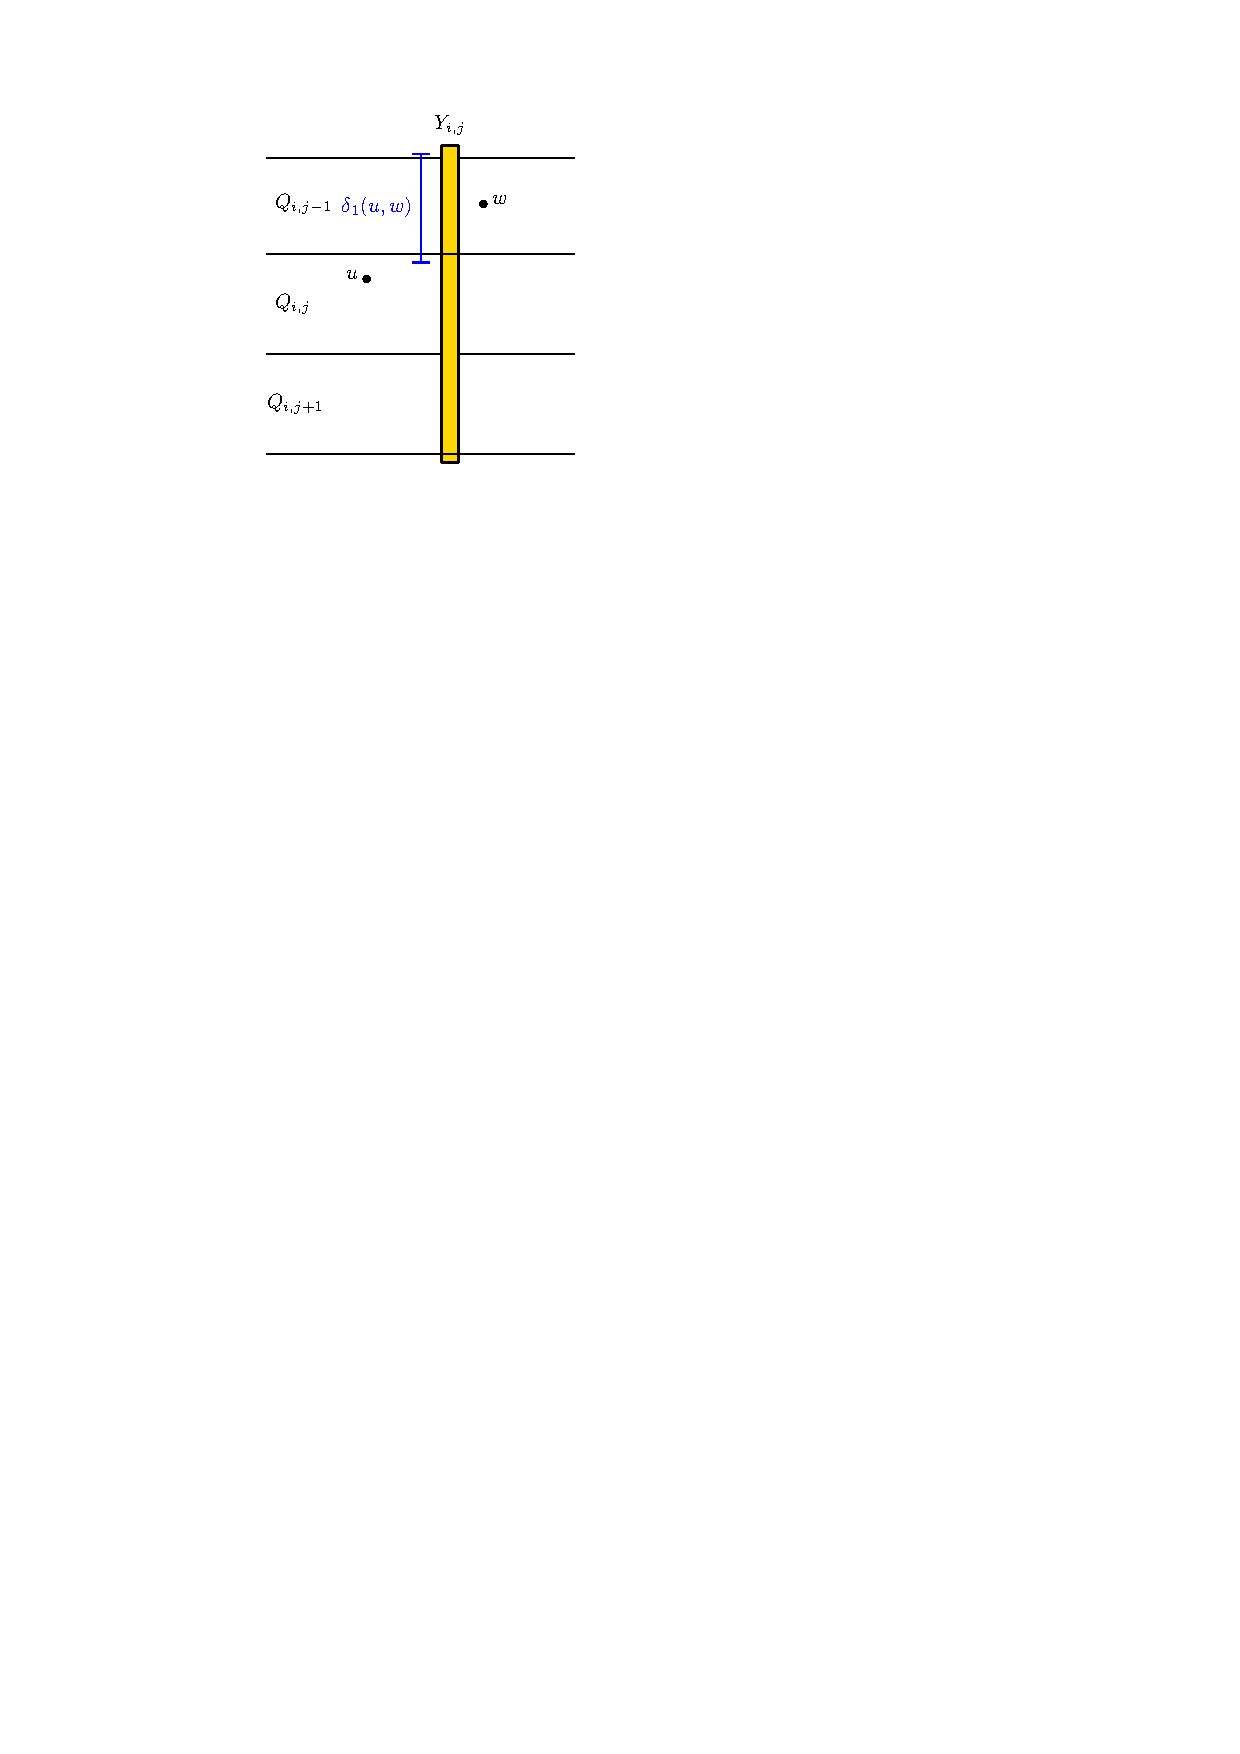
\includegraphics[page=1,scale=0.9]{figs/new_metric} &
    \includegraphics[page=2,scale=0.9]{figs/new_metric} &
    \includegraphics[page=3,scale=0.9]{figs/new_metric}
    \end{tabular}
    \caption{The definitions of $\delta_1$, $\delta_2$, and $\delta_3$.}
    \label{d_star}
\end{figure}

Ultimately, $d^*$ will be the maximum of several functions, one of which is $\delta_0$.  Of these functions, $\delta_0$ is the most important because it ensures that the metric space $\mathcal{M}^*$ has local density $O(D)$.

\begin{lem}\label{delta_density}
  For each $v\in V(H\boxtimes P)$ and $r\ge 1$,
  \[
    |B_{(V(G),\delta_0)}(v,r):=\{w\in V(G):\delta_0(v,w)\le r\}| \le 3Dr \enspace .
  \]
\end{lem}

\begin{proof}
  Since $\delta_0(v,w)$ is always zero or an integer power of $2$, we may assume that $r=2^k$ for some integer $k$.  If $\delta_0(v,w)\le r$ for some $w\in V(G)$, then $v$ and $w$ are in the same component of $Q^+_{i,j}-X_{i,j}$ for some $i \le k$.  For each $i\in\{0,\ldots,k\}$, there are three values of $j$ such that $v\in V(Q^+_{i,j})$.  For each of these, the component of $Q^+_{i,j}-X_{i,j}$ that contains $v$ has at most $D2^{i-1}$ vertices of $G$. Therefore,
  \[
    |B_{(V(G),d^*)}| \le |\{w\in V(G): \delta_0(v,w)\le r\}| \le \sum_{i=0}^{k-1} 3D2^{i} = 3D(2^{k}-1) < 3Dr \enspace . \qedhere
  \]
\end{proof}

By \cref{delta_density}, $\delta_0$ defines a space $(V(G),\delta_0)$ with local density $O(D)$.  Unfortunately, this is not a metric space because $\delta_0$ does not necessarily satisfy the triangle inequality.  The remaining functions used to define $d^*$ are used to ensure that $d^*$ is a metric space.

Let $v:=(x_2,y_b)$.  We now define a second quantity $\mathdefin{\delta_1(v,w)}$.  If there exists some $i\in\{0,\ldots\log N\}$ such that $v,w\in V(G_{i,j})$ but $v$ and $w$ are in different components of $G_{i,j}-X_{i,j+1}$ then let $i_1(v,w)$ be the maximum such $i$ and set $\delta_1(v,w)=b-j2^i + c-j2^i$. If no such $i$ exists, then let $i_1(v,w):=-\infty$ and $\delta_1(v,w):=0$.

The third quantity $\mathdefin{\delta_2(v,w)}$ is defined symmetrically: If there exists some $i\in\{0,\ldots\log N\}$ such that $v,w\in V(G_{i,j})$ but $v$ and $w$ are in different components of $G_{i,j}-X_{i,j-1}$ then let $i_2(v,w)$ be the maximum such $i$ and set $\delta_2(v,w)=(j+1)2^i-b + (j+1)2^i-c$. If no such $i$ exists, then let $i_2(v,w):=-\infty$ and $\delta_2(v,w):=0$.

From the definition of $i_1$ and $i_2$ we immediately obtain the following property, which will be useful later.

\begin{obs}\label{i_bounds}
  For each $b\in\{1,2\}$, if
  $i_b(v,w)\ge 0$ then $\delta_b(v,w)\le 2^{i_b(v,w)+1}$.
\end{obs}

Finally, define
\[
  \mathdefin{d^*(u,w)} := \max\{\delta_0(u,w),\, \delta_1(u,w),\, \delta_2(u,w),\, d_{H\boxtimes P}(u,w) \}
\]
First we argue that $d^*$ is a contraction of $d_{(H\boxtimes P)-X}$.
\begin{lem}\label{d_star_contraction}
  For any pair of vertices $u,v,\in V((H\boxtimes P)-X)$, $d^*(u,v)\le d_{(H\boxtimes P)-X}(u,v)$.
\end{lem}

\begin{proof}
  If $\delta_0(u,v)=2^i$ because, say $i_0(u,v)=i$, then any path in $(H\boxtimes P)-X$ from $u$ to $v$ must begin in the subgraph $Q_{i,j}$ that contains $u$ and must not be contained in the subgraph $Q^+_{i,j}$.  Therefore $d_{(H\boxtimes P)-X}(u,v) \ge 2^i=\delta_0(u,v)$.

  If $\delta_1(u,v)=p>0$ and $i_1(u,v)=i$, then any path from $u$ to $v$ must begin at $u$, leave the subgraph of $H\boxtimes P$ induced by $V(Q_{i,j})\cup V(Q_{i,j+1})$ and return to $v$.  The shortest such path contains at least $\delta_1(u,v)$ vertices in $V(Q_{i,j})\cup V(Q_{i,j+1})$ plus one additional vertex.  Therefore $d_{(H\boxtimes P)-X}(u,v) \ge \delta_1(u,v)$.  The argument for $\delta_2$ is symmetric.
\end{proof}

Next we argue that $d^*$ is a distance function.

\begin{lem}\label{d_star_metric}
  The function $d^*$ is a distance function for $V(H\boxtimes P)\setminus X$.
\end{lem}

\begin{proof}
  It is straightforward to verify that $d^*(u,u)=0$ for all $u\in V(H\boxtimes P)\setminus X$ and that $d^*(u,v)=d^*(v,u)\ge 0$ for all $u,v\in V(H\boxtimes P)\setminus X$.  All that remains is to verify that $d^*$ satisfies the triangle inequality.

  Let $u:=(x_1,y_a)$, $v:=(x_2,y_b)$ and $w:=(x_3,y_c)$ be three vertices of $(H\boxtimes P)- X$.  We must show that $d^*(u,w)\le d^*(u,v)+d^*(v,w)$.  If $d^*(u,w)=0$ then this is immediate, so suppose $d^*(u,w)>0$.

  If $d^*(u,w)=d_{H\boxtimes P}(u,w)$ then this follows immediately from the fact that $d_{H\boxtimes P}$ satisfies the triangle inequality and the fact that $d^*(u,v) + d^*(v,w)\ge d_{H\boxtimes P}(u,v)+d_{H\boxtimes P}(v,w)$.

  Otherwise, if $d^*(u,w)=\delta_0(u,w)$ then
  $i_0(u,w)\ge 0$. Assume, without loss of generality that $i:=i_0(u,w)=i_0^{\shortrightarrow}(u,w)$.  Let $j$ be such that $Q_{i,j}$ contains $u$.  Then $u$ and $w$ are in different components, $C_u$ and $C_w$ of $Q^+_{i,j}-X_{i,j}$.  We distinguish between two cases depending on the location of $v$.  If $v$ is not a vertex of $Q^+_{i,j}$, then $d_{(H\boxtimes P)-X}(u,v) \ge d_{H\boxtimes P}(u,v) \ge 2^i=\delta_0(u,w)$ and there is nothing to prove.  Otherwise, $v$ is contained in some component $C_v$ of $Q^+_{i,j}-X_{i,j}$.  If $C_v\neq C_u$ then $i_0(u,v)\ge i$ so $d^*(u,v)\ge 2^i$ and again there is nothing to prove.  If $C_v=C_u$, then $d^*(u,v)+d^*(v,w)\ge d_{H\boxtimes P}(u,v)+\delta_b(v,w)\ge 2^i=d^*(u,w)$ for some $b\in\{0,1,2\}$.

  Finally, we consider the case where $d^*(u,w)=\delta_1(u,w)$. Then $i:=i_1(u,w)\ge 0$, so $u$ and $w$ are both contained in $G_{i,j}$ but in different components $C_u$ and $C_w$ of $G_{i,j}-X_{i,j+1}$, for some $j$.  If $v$ is not a vertex of $G_{i,j}$ then $d^*(u,v)+d^*(v,w)\ge d_{H\boxtimes P}(u,v)+d_{H\boxtimes P}(v,w) \ge \delta_1(u,w)$ and we are done.  If $v$ is a vertex of $C_u$, then $d^*(u,v)+d^*(v,w)\ge d_{H\boxtimes P}(u,v)+\delta_1(v,w)\ge \delta_1(u,w)$. The case where $v$ is a vertex of $C_w$ is symmetric.  If $v$ is neither a vertex of $C_u$ nor a vertex of $C_w$, then $d^*(u,v)+d^*(v,w)\ge \delta_1(u,v) + \delta_1(v,w) \ge \delta_1(u,w)$.
\end{proof}


The preceding lemmas are summarized in the following corollary:

\begin{cor}
  The metric space $(V((H\boxtimes P)-X), d^*)$ is a is a contraction of $(V((H\boxtimes P)-X), d_{(H\boxtimes P)-X})$ and the metric space $(V(G-X),d^*)$ has local density $O(D)$.
\end{cor}



\subsection{Volume-Preserving Contraction of $\mathcal{M}^*$}

In this section we prove the following result:

\begin{lem}\label{dstar_contraction}
  For every integer $k\in\{1,\ldots,n\}$, the metric space $\mathcal{M}^*:=(V(G-X),d^*)$ has a $(k,O(\sqrt{\log n}))$-volume-preserving Euclidean contraction. \todo{Check quantifier on $k$}
\end{lem}

\subsection{Decomposing $H$: The Klein-Plotkin-Rao Partition}

\pat{The next two sections can be simplified.  We can assume $H$ is a $t$-tree.  Then doing BFS in $H$ and chopping one out of every $\Delta$ layers breaks $H$ into components of weak diameter at most $2\Delta$ (by shadow completeness).  Then you chop $P$ as before, which breaks $H\boxtimes P$ into components of weak diameter at most $2\Delta$.}


First, fix some integer $\Delta \ge 1$.
Consider the following random process that, given a connected graph $H$ constructs a random subset $\mathdefin{\textsc{Chop}_{\Delta,t}(H)}$ of vertices in $H$. If $t=0$ then $\textsc{Chop}_{\Delta,0}(H):=\emptyset$.  Otherwise, select any vertex $x$ in $H$ and choose a uniformly random $r\in\{0,\ldots,\Delta-1\}$.  Let $R:=\{y\in V(H):d_{H}(x,y)\equiv r\pmod{\Delta}\}$ and let $C_1,\ldots,C_m$ be the connected components of $H-R$.  Then $\textsc{Chop}_{\Delta,t}(H):=R\cup\bigcup_{i=1}^m \textsc{Chop}_{\Delta,t-1}(C_i)$.


The following lemma, with a greater dependence on $t$, is due to \citet{klein.plotkin.ea:excluded}. The version shown here was proved by \citet{fakcharoenphol.talwar:improved}. The presentation here closely follows that of \citet{lee:simpler}.

\begin{lem}[{\citet{klein.plotkin.ea:excluded,fakcharoenphol.talwar:improved,lee:simpler}}]\label{component_diameter_h}
  If $H$ is a connected $K_{t+1}$-minor-free graph then each component $C$ of $H-\textsc{Chop}_{\Delta,t}(H)$ has $\diam_H(C)\le 16t\Delta$.
\end{lem}


% Say that a vertex $x$ of $H$ is \defin{$\delta$-good} with respect to a set $X\substeq V(H)$ if $d_{H}(x,X)\ge \delta$ and $x$ is \defin{$\delta$-bad} with respect to $X$ otherwise.

% In the following lemma, and for the rest of this section, we use the convention that for any vertex $x$ of $H$, $d_H(x,\emptyset):=\infty$.

\begin{lem}\label{delta_bad_h}
  For any vertex $x$ of $H$ and any integer $\delta\ge 1$, $$\Pr(d_H(x, \textsc{Chop}_{\Delta,t}(H)< \delta)\le t\,(2\delta-1)/\Delta.$$
\end{lem}

\begin{proof}
  The proof is by induction on $t$. If $d_H(x,\textsc{Chop}_{\Delta,t}(H) < \delta)$ then $d(x,R)< \delta$ or, if $t>1$,  $d_H(x,\textsc{Chop}_{\Delta,t-1}(C) < \delta)$ where $C$ is the component of $H-R$ that contains $x$.  Since there are at most $2\delta-1$ choices of $r$ for which $d_H(x,R)<\delta$, $\Pr(d_H(x,R)<\delta) \le (2\delta-1)/\Delta$. For $t=1$, this completes the proof.  For $t>1$, the proof follows from the inductive hypothesis on $\textsc{Chop}_{\Delta,t-1}(C)$ and the union bound.
\end{proof}

\subsection{\boldmath Decomposing $H\boxtimes P$}

% Let $G$ be a subgraph of $H\boxtimes P$ where $P:=y_1,\ldots,y_h$.

Choose a uniformly random $r_0\in\{0,\ldots,\Delta-1\}$, let $Y_0:=Y_{0,\Delta,t}(P):=\{y_i\in V(P):i\equiv r_0\pmod\Delta\}$ and let $Y:=Y_{\Delta,t}(P):=V(H)\times Y_0$.  Let $W_0\subseteq V(H)$ be the set obtained by executing $\textsc{Chop}_{\Delta,t}(H)$, let $W:=W_0\times V(P)$ and let $Z:=\mathdefin{Z_{\Delta,t}(H,P)}:=W\cup Y$.

% For some intuition, it is helpful to consider the case when $H$ is a path and $t=1$.  In this case, $H\boxtimes P$ is a grid with diagonal edges.  Starting from row $r\in\{0,\ldots,\Delta-1\}$, the set $Y$ contains one out of every $\Delta$ rows of this grid.  Each of the components $C_1,\ldots,C_m$ of $H\boxtimes P-Y$, except the top-most, $C_1$ and bottom-most, $C_m$ is a grid with $\Delta-1$ rows.  For each component $C_i$, the set $X$ contains one out of every $\Delta$ columns of $C_i$, starting from column $r_i\in\{0,\ldots,\Delta-1\}$. \todo{Add figure}

\begin{lem}\label{component_diameter}
  If $H$ is $K_{t+1}$-minor-free, then each component $C$ of $H\boxtimes P-Z$ has $\diam_{H\boxtimes P}(C)\le ?t\Delta$.
\end{lem}

\begin{proof}
  Let $C$ be a component of $H\boxtimes P-Z$.  For any two vertices $x:=(x_1,x_2)$ and $y:=(y_1,y_2)$ of $C$, $d_{H\boxtimes P}(x,y) = \max\{d_{H}(x_1,y_1),d_{P}(x_2,y_2)$. By \cref{component_diameter_h},  $d_{H\boxtimes P}(x_1,y_1)\le ?t\Delta$.  By the choice of $Y_0$, $d_{P}(x,y)<\Delta$.
\end{proof}

\begin{lem}\label{delta_bad_product}
  For any vertex $x$ of $H\boxtimes P$ and any integer $\delta\ge 1$, $$\Pr(d_{H\boxtimes P}(x,Z)< \delta)\le (t+1)(2\delta-1)/\Delta.$$
\end{lem}

\begin{proof}
  If $d_{H\boxtimes P}(x,Z)<\delta$ then $d_{H\boxtimes P}(x,Y)<\delta$ or $d_{C}(x,Z)<\delta$ where $C$ is the component of $H\boxtimes P-Y$ that contains $x$.  Again, there are at most $2\delta-1$ choices of $r_0$ for which $d_{H\boxtimes P}(x,Y)<\delta$, so $\Pr(d_{H\boxtimes P}(x,Y)<\delta)\le (2\delta-1)/\Delta$.  The proof now follows from the union bound and \cref{delta_bad_h}.
\end{proof}


% \subsection{\boldmath Decomposing $Q_{i,j}-X_{i,j}$}
%
% Let $C$ be a component of $Q_{i,j}-X_{i,j}$ for some $i\ge 1$ and some $j$.  Then $C=H'\boxtimes P_{i,j}$ where $H'$ is a subgraph of $H$ (a component of $H-X'_{i,j}$) and $P_{i,j}=y_{(i-1)2^i+1},\ldots,y_{(i+1)2^i}$ is a subpath of $P$ with $3\cdot2^i$ vertices.  Choose a uniformly random $r_0\in\{0,\ldots,\Delta-1\}$, let $A_0:=\{y_{(i-1+a)2^i+1+r_0}: a\in\{0,1,2\}\}$ and let $A:=A(C):=V(H')\times A_0$.  Let $P_1,P_2,P_3$ be the components (each of which is a path) of $P-Y_0$ and let $B_1,B_2,B_3$ be the results of independent executions of $\textsc{Chop}_{2^i,t}(H')$ and let $B:=B(C):=\bigcup_{i=1}^3 V(P_i)\times B_i$.  Finally, let $Z:=Z(C):=B\cup Y$.
%
% % For some intuition, it is helpful to consider the case when $H$ is a path and $t=1$.  In this case, $H\boxtimes P$ is a grid with diagonal edges.  Starting from row $r\in\{0,\ldots,\Delta-1\}$, the set $Y$ contains one out of every $\Delta$ rows of this grid.  Each of the components $C_1,\ldots,C_m$ of $H\boxtimes P-Y$, except the top-most, $C_1$ and bottom-most, $C_m$ is a grid with $\Delta-1$ rows.  For each component $C_i$, the set $X$ contains one out of every $\Delta$ columns of $C_i$, starting from column $r_i\in\{0,\ldots,\Delta-1\}$. \todo{Add figure}
%
% \begin{lem}\label{component_diameter}
%   Each component of $C-Z$ has diameter at most $?t2^i$.
% \end{lem}
%
% \begin{proof}
%   Let $C'$ be a component of $C-Z$.  For any two vertices $x:=(x_1,x_2)$ and $y:=(y_1,y_2)$ of $C'$, $d_{C}(x,y) = \max\{d_{H'-B_j}(x_1,y_1),d_{P'}(x_2,y_2)$ where $B_j$ is the result of running $\textsc{Chop}_{\Delta,t}(H')$. By \cref{component_diameter_h},  $d_{H-X_j}(x_1,y_1)\le ?t\Delta$.  By the choice of $Y_0$, $d_{P}(x,y)<\Delta$.
% \end{proof}
%
%
% \begin{lem}\label{delta_bad_product}
%   For any vertex $x$ of $C$ and any integer $\delta\ge 1$, $\Pr(d_{C}(x,Z)< \delta)\le (t+1)(2\delta-1)/\Delta$.
% \end{lem}
%
% \begin{proof}
%   If $d_{C}(x,Z)<\delta$ then $d_{C}(x,A)<\delta$ or $d_{C}(x,B)<\delta$ where $C$ is the component of $H\boxtimes P-Y$ that contains $x$.  Again, there are at most $2\delta-1$ choices of $r_0$ for which $d_{C}(x,A)<\delta$, so $\Pr(d_{C}(x,A)<\delta)\le (2\delta-1)/\Delta$.  The proof now follows from the union bound and \cref{delta_bad_h}.
% \end{proof}

% \Cref{delta_bad_product} with $\delta=1$ yields the following results:
%
% \begin{cor}
%   For any $x\in V(H\boxtimes P)$, $\Pr(x\in Z)\le (t+1)/\Delta$.
% \end{cor}
%
% I don't think this is relevant.

\subsection{\boldmath The Mapping $\phi$}

Let $Z:=Z_{\Delta,t}(H,P)$ be a subset of $V(H\boxtimes P)$ generated by running the procedure described above, for some $\Delta\in\{1,\ldots,|V(P)|\}$.\footnote{The assumption $\Delta\le |V(P)|$ ensures that $Z$ is non-empty, so that $d_{H\boxtimes P}(x,Z)<\infty$ for all $x\in V(H\boxtimes P)$.}  Consider the graph $I:=\mathdefin{I(Z)}$ obtained from $Q\boxtimes P$ by removing all edges incident to at least one vertex in $Z$.

For each component $C$ of $I$, let $X_C:=\cup\{X_{i,j}:C\subseteq Q^+_{i,j},\, i\in\{0,\ldots,\log N\}, j\in\{0,\ldots,N/2^i-1\}\}$.  In words, $X_C$ contains only the vertical cuts used to construct $X$ that cut $C$ from top to bottom. Let $J$ be the subgraph of $I$ obtained by removing, for each component $C$ of $I$, the vertices in $X_C\cap V(C)$.

\begin{lem}\label{dstar_component_diameter}
  Each component $C'$ of $J$ has $\diam_{d^*}(C')\le ?t\Delta$.
\end{lem}

\begin{proof}
  Let $C'$ be component of $J$. Let $C$ be the component of $I$ that contains $C'$. Let $v$ and $w$ be two vertices of $C'$. We need to show that $d(v,w)\le ?t\Delta$ for each $d\in\{\delta_0, \delta_1,\delta_2,d_{H\boxtimes p}\}$.

  Since $v$ and $w$ are both in $C$, \cref{component_diameter} implies that $d_{H\boxtimes P}(v,w)\le ?t\Delta \le ?t\Delta$.

  Suppose, for the sake of contradiction, that $\delta_0(v,w)=2^i> ?t\Delta> \Delta$. Then, for some $j$, $v\in V(Q_{i,j})$,  $w\in V(Q^+_{i,j})$, and $v$ and $w$ are in different components of $Q^+_{i,j}-X_{i,j}$.  Since $2^i>\Delta$, $Q^+_{i,j}$ contains $C$ so $X_C$ contains $X_{i,j}$. Therefore, $v$ and $w$ are in different components of $C-X_C$, contradicting the assumption that $v$ and $w$ are in the same component of $J$.

  Suppose, for the sake of contradiction, that $\delta_1(v,w)>?t\Delta \ge 2\Delta$.  Then, for some $j$, $v$ and $w$ are vertices of $Q_{i,j}$ that are in different components of $X_{i,j+1}$. Since $\delta_1(v,w)>2\Delta$ and $C$ contains both $v$ and $w$, $Q^+_{i,j+1}$ contains $C$. Again, this contradicts the assumption that $v$ and $w$ are in the same component of $J$.  The situation in which $\delta_2(v,w)>?t\Delta$ is handled symmetrically.
\end{proof}




%
%
% \begin{lem}\label{different_components}
%   Let $v$ and $w$ be two vertices of $(H\boxtimes P)-X$.  If $d^*(v,w)>?t\Delta$ then $v$ and $w$ are in different components of $I-X$.
% \end{lem}
%
% \begin{proof}
%   If either of $v$ or $w$ are in $Z$, then this vertex is an isolated vertex in $I$ and the result is trivial. Therefore, we may assume that $v,w\in V((H\boxtimes P)-(X\cup Z))$.  Then, exactly one of the following cases applies:
%   \begin{compactenum}
%     \item $d^*(v,w)=d_{H\boxtimes P}(v,w)$.  In this case, \cref{component_diameter} implies that $v$ and $w$ are in different components of $Z$.
%     \item $d^*(v,w)=\delta_0(v,w)$.  This implies that, for $i:=i_0(v,w)$, and some $j$, $d^*(v,w)=2^i$, and $v$ and $w$ are vertices of $Q_{i,j}$ that are in different components of $Q^+_{i,j}-X_{i,j}$.  Let $Y=V(H)\times Y_0\subseteq Z$ be as in the definition of the set $Z$.  Since $2^i\ge ?t\Delta\ge \Delta$, any component of $(H\boxtimes P)-Y$ that contains $v$ and $w$ is contained in $Q^+_{i,j}$.  Since $v$ and $w$ are in different components of $Q^+_{i,j}-X_{i,j}$, they are in different components of $H\boxtimes P-(X_{i,j}\cup Y)\supseteq (H\boxtimes P)-(X\cup Z)$.
%     \item $d^*(v,w)=\delta_1(v,w)$ or $d^*(v,w)=\delta_1(v,w)$.  Since these two cases are symmetric, we may assume without loss of generality that $d^*(v,w)=\delta_1(v,w)$.   This implies that, for $i:=i_1(v,w)$ and some $j$, $v$ and $w$ are vertices of $Q_{i,j}$ that are in different components of $Q_{i,j}-X_{i,j+1}$. This implies that $v$ and $w$ are both contained in $Q^+_{i,j+1}$ but are in different components of $Q^+_{i,j+1}-X_{i,j+1}$.  By the definition of $\delta_2$, $d_{H\boxtimes P}(x,V(H\boxtimes P-V(Q_{i,j})))\ge d^*(v,w)/2\ge ?t\Delta/2\ge\Delta$ for at least one $x\in\{v,w\}$. Without loss of generality, suppose $x=v$.  Then the component of $(H\boxtimes P)-Y$ that contains $v$ is contained in $Q^+_{i,j+1}$.  Since $v$ and $w$ are in different components of $Q^+_{i,j+1}-X_{i,j+1}$, they are in different components of $H\boxtimes P-(X_{i,j+1}\cup Y)\supseteq (H\boxtimes P)-(X\cup Z)$. \qedhere
%   \end{compactenum}
% \end{proof}

For each component $C'$ of $J$, choose a uniformly random $\alpha_{C'}$ in $[0,1]$, with all choices made independently. For each component $C'$ and each $v \in V(C')$, let
\[
  \varphi_{Z}(v):=(1+\alpha_{C'})\,d^+_{H\boxtimes P}(v,Z) \enspace .
\]
(Note that this definition uses positive distance $d^+_{H\boxtimes P}$.)


% Let $i^*:=2^{\lceil\log\Delta\rceil}$ and let \
% \[
%   X_{\ge i^*}:=\bigcup_{i=i^*}^{\log N}\bigcup_{j=0}^{N/2^i-1} X_{i,j} \enspace .
% \]
% Let $C_1,\ldots,C_p$ be the components of $I-X_{i^*}$, let $\alpha_1,\ldots,\alpha_p$ be mutually independent uniform real numbers in $[0,1]$, and let $\varphi_{Z}(x):=(1+\alpha_i)\,d_{H\boxtimes P}(x,Z)$, for each $x\in C_i$ and each $i\in\{1,\ldots,p\}$.
% (Note that this definition uses positive distance $d^+_{H\boxtimes P}$.)


\begin{obs}\label{uniform}
  For fixed $Z:=Z_{\Delta,t}(H,P)$, $\varphi_Z(v)$ is uniformly distributed in $[d^+_{H\boxtimes P}(v,Z), 2d^+_{H\boxtimes P}(v,Z)]$, for each $v\in V(H\boxtimes P)$.
\end{obs}


\begin{lem}\label{double_distance}
  For any two vertices $v,w\in V(H\boxtimes P)\setminus X$,
  \[
    |\varphi_Z(v)-\varphi_Z(w)| \le 12 d^*(v,w) \enspace .
  \]
\end{lem}

\begin{proof}
  If $v=w$ then $|\varphi_Z(v)-\varphi_Z(w)|=0 = 2 d^*(v,w)$, so we assume $v\neq w$.

  First we deal with the issues caused by using $d^+_{H\boxtimes P}$ rather than $d_{H\boxtimes P}$.  If $v$ and $w$ are both in $Z$ then, for some $\alpha_v,\alpha_w\in [0,1]$,  $|\varphi_Z(v)-\varphi_Z(w)|=|(1+\alpha_v)-(1+\alpha_w)|\le 1 \le d_{H\boxtimes P}(v,w)\le d^*(v,w)$.  If $v\not\in Z$ and $w\in Z$ (or vice-versa), then $|\varphi_Z(v)-\varphi_Z(w)|= |(1+\alpha_v)d_{H\boxtimes P}(v,Z)-(1+\alpha_w)|\le 2d_{H\boxtimes P}(v,Z)-1\le 2d_{H\boxtimes P}(v,w)-1< 2d^*(v,w)$.  Therefore, we may assume that neither $v$ nor $w$ is in $Z$.

  Observe that, if $\Delta=1$, then $Z=V(H\boxtimes P)$ and we are already done, so we now assume that $\Delta\ge 2$.  If $v$ and $w$ are in different components of $I$ then
  \begin{align*}
     |\varphi_Z(v)-\varphi_Z(w)|
    & =|(1+\alpha_v)d_{H\boxtimes P}(v,Z)-(1+\alpha_w)d_{H\boxtimes P}(w,Z)| \\
    & < 2\max\{d_{H\boxtimes P}(v,Z), d_{H\boxtimes P}(Z,w)\} \\
    & \le 2\left(d_{H\boxtimes P}(v,Z) + d_{H\boxtimes P}(Z,w)\right) \\
    & \le 2d_{H\boxtimes P}(v,w) \le 2d^*(v,w) \enspace ,
  \end{align*}
  where the penultimate inequality follows from the fact that every path in $H\boxtimes P$ from $v$ to $w$ contains at least one vertex in $Z$.  We now assume that $v$ and $w$ are in the same component of $I$.

  If $v$ and $w$ are in the same component $C'$ of $J$ then
  \begin{align*}
    |\varphi_Z(v)-\varphi_Z(w)|
    & =(1+\alpha_{C'})|d_{H\boxtimes P}(v,Z)-d_{H\boxtimes P}(w,Z)| \\
    & \le 2|d_{H\boxtimes P}(v,Z)-d_{H\boxtimes P}(w,Z)| \\
    & \le 2 d_{H\boxtimes P}(v,w) \le 2d^*(v,w) \enspace ,
  \end{align*}
  where the penultimate inequality is obtained by rewriting the triangle inequalities $d(v,Z)\le d(v,w)+d(w,Z)$ and $d(w,Z)\le d(w,v)+d(v,Z)$.

  All that remains is to consider the case where $v$ and $w$ are in the same component $C$ of $I$ but in different components $C_v$ and $C_w$ of $J$.  Then there exists some $i$ and $j$ such that $C$ is contained in $Q^+_{i,j}$ but $v$ and $w$ are in different components of $Q^+_{i,j}-X_{i,j}$.  Since $C$ is contained in $Q^+_{i,j}$, $3\cdot 2^{i} \ge \Delta-1\ge \Delta/2$.
  \begin{compactitem}
    \item If one of $v$ or $w$, say $v$, is in $Q_{i,j}$ then $i_0(v,w)\ge i$, so $d^*(v,w)\ge \delta_0(v,w)\ge 2^i\ge \Delta/6$.
    \item If $v$ and $w$ are both in $G_{i,j-1}$ or both in $G_{i,j+1}$ then $\delta_1(v,w)\ge d_{H\boxtimes P}(v,Z)+d_{H\boxtimes P}(w,Z)$, since $d_{H\boxtimes P}(v,\overline{C})\le d_{H\boxtimes P}(v,\overline{V(Q^+_{i,j+1})})$.
    \item If one of $v$ or $w$ is in $G_{i,j-1}$ and the other is in $G_{i,j+1}$, then $d_{H\boxtimes P}(v,w)\ge 2^i\ge\Delta/6$.
  \end{compactitem}
  Since $d_{H\boxtimes P}(v,Z)\le \Delta/2$ and $d_{H\boxtimes P}(w,Z)\le \Delta/2$, each of the three cases implies that
  \[
    d^*(v,w) \ge \Delta/6 \ge (d_{H\boxtimes P}(v,Z) + d_{H\boxtimes P}(w,Z))/6 \enspace .
  \]
  We finish with
  \begin{align*}
      |\varphi_Z(v)-\varphi_Z(w)|
      & =|(1+\alpha_{C_v})d_{H\boxtimes P}(v,Z)-(1+\alpha_{C_w})d_{H\boxtimes P}(w,Z)| \\
      & \le 2\max\{d_{H\boxtimes P}(v,Z), d_{H\boxtimes P}(Z,w)\} \\
      & \le 2\left(d_{H\boxtimes P}(v,Z) + d_{H\boxtimes P}(Z,w)\right) \\
      & \le 12\, d^*(v,w) \enspace . \qedhere
  \end{align*}
\end{proof}

Let $a$ be a constant whose value will be lower-bounded later.  We now define a random function $\phi:V(G)\to\R^{L}$ where $L:=\lfloor 1+\log_2 n\rfloor\cdot\lceil a k\ln n\rceil$. For each $i\in\{0,\ldots,\log N-1\}$ each $j\in\{1,\ldots,\lceil a k\ln n\rceil\}$, let $Z_{i,j}\sim Z_{\Delta,t}(H,P)$ be the random subset of $V(H\boxtimes P)$ obtained by using the procedure described above with parameters $\Delta=2^i$ and $t$ and with all random choices made independently.  For each $x\in V(H\boxtimes P)-X$, we set $\phi_{i,j}(x):= \varphi_{Z_{i,j}}(x)$, again with all choices made independently.

Finally, define
\[
   \phi(x) := \left(\phi_{i,j}(x):(i,j)\in \{0,\ldots,\lfloor \log_2 n\rfloor\}\times\{1,\ldots,\lceil a k\ln n\rceil\}\right) \enspace .
\]


The following lemma says that $\phi$ is almost a Euclidean contraction of $(V(H\boxtimes P)\setminus X,d^*)$.  In a final step, we will divide each coordinate of $\phi$ by $12\sqrt{L}$ to obtain a Euclidean contraction but, until then, it is more convenient to work directly with $\phi$.

\begin{lem}\label{euclidean_contraction}
  For each $v,w\in V((H\boxtimes P)-X)$, $$d_2(\phi(v),\phi(w)) \le 12\sqrt{L}\cdot d^*(v,w).$$
\end{lem}

\begin{proof}
  By \cref{double_distance}, $|\phi_{i,j}(v)-\phi_{i,j}(w)|\le 12d^*(v,w)$ for each $(i,j)\in\{0,\ldots,\log N\}\times\{1,\ldots,\lceil ak\ln n\rceil\}$.  Therefore,
  \[
    d_2(\phi(v),\phi(w)) = \left(\sum_{i,j}(\phi_{i,j}(v)-\phi_{i,j}(w))^2\right)^{1/2}
    \le \left(L (12d^*(v,w))^2\right)^{1/2} = 12\sqrt{L}d^*(v,w) \enspace . \qedhere
  \]
\end{proof}


% \pat{This paragraph should be turned into a lemma.} Although $\phi$ maps vertices of $H\boxtimes P$ to $\R^L$, it is not necessarily a Euclidean contraction: $\phi$ has $L$ coordinates and for two vertices $x$ and $y$, the difference between $\phi_{i,j}(x)$ and $\phi_{i,j}(y)$ can be as much as $2d_{H\boxtimes P}(x,y)$ (but not more).  Thus, $d_2(\phi(x),\phi(y))$ can exceed $d_{H\boxtimes P}(x,y)$ by a factor of up to $2\sqrt{L}$ (but not more).  In a final step, we will divide each coordinate of $\phi$ by $2\sqrt{L}$ but, until then, it is more convenient to work with $\phi$.

% For a reader familiar with \cite{rao:small}, the preceding discussion will look familiar, and may give the impression that the only significant difference is the extra level of chopping (by choosing $r_0$) needed to deal with the factor $P$ in the product $H\boxtimes P$. Indeed, making only those modifications would give a $(k,O(\sqrt{n}))$-volume preserving embedding of $(V(G),d_{H\boxtimes P})$. This not good enough, though, because there is no upper bound on the local density of $(V(G),d_{H\boxtimes P})$, which is why we will show that $\phi$ gives a  $(k,O(\sqrt{n}))$-volume preserving embedding of $(V(G),d^*)$.  At first glance, this is surprising, since $\phi$ is always defined entirely in terms of $d_{H\boxtimes P}$.  Ultimately, what makes this work is the fact that each component $C'$ of $J$ is assigned its own random value $\alpha_{C'}$.
% If $d^*(v,w)$ is a bit larger than $2^i$ but $d_{H\boxtimes P}(v,w)$ is much smaller than $2^i$, then $v$ and $w$ are in different components of $G_{i,j}-X$.  Roughly, this ensures that $\phi_{i,j}(v)$ and $\phi_{i,j}(w)$ are sufficiently independent to ensure that their expected difference is $\Omega(2^i)$.


The rest of the analysis in this section closely follows \citet{rao:small}, which in turn closely follows \citet{feige:approximating}.  The main difference is that we work with $d^*$ rather than $d_G$.  We proceed slowly and carefully since our setting is significantly different and we expect that many readers will not be familiar with some methods introduced by \citet{feige:approximating} that are only sketched by \citet{rao:small}.

We make use of this simple \defin{Chernoff Bound}:  For a $\operatorname{binomial}(n,p)$ random variable $B$ and any $0<\delta<1$, $\Pr(B \le np/2) \le \exp(-np/8)$.

Let $\Gamma_k:=\{(\lambda_1,\ldots,\lambda_k)\in \R^k:\sum_{j=1}^k\lambda_j=1\}$, that is, $\Gamma_k$ is the set of coefficients that can be used to obtain an affine combination of $k$ numbers.  In the following lemma, which is the crux of the proofs in \cite{rao:small,feige:approximating} it is critical that the function $\lambda$ chooses an affine combination $\lambda_1,\ldots,\lambda_{p-1}$ by only considering $\phi(v_1),\ldots,\phi(v_{p-1})$.  Thus any dependence between $\lambda_1,\ldots,\lambda_{p-1}$ and $\phi(v_p)$ is limited to random choices made during the construction of $\phi$ that get used to define $\phi(v_1),\ldots,\phi(v_{p-1})$.


\begin{lem}\label{crux}
  Fix some function $\lambda:(\R^{L})^{p-1}\to \Gamma_{p-1}$.
  % Let $G$, $H\boxtimes P$, $X$,  be $K_{t+1}$-minor-free graph with at most $n$ vertices, let $P$ be a path with at most $n$ vertices, and let $\phi:V(H\boxtimes P)\to\R^L$ be the probabilistic embedding defined above. In particular, the random choices made in the construction of $\phi$ are independent of $\lambda$.
  Let $v_1,\ldots,v_p$ be distinct vertices of $(H\boxtimes P)-X$ and let $h:=d^*(v_p,\{v_1,\ldots,v_{p-1}\})$.  Let $(\lambda_1,\ldots,\lambda_{p-1}):=\lambda(\phi(v_1),\ldots,\phi(v_{p-1}))$ and let $x:=\sum_{j=1}^{p-1}\lambda_j\phi(v_j)$.
  Then, with probability at least $1-n^{-3k}$,
  \[
    d_2(\phi(v_p),x)\ge \frac{h\sqrt{ak\ln n}}{160?(t+1)} \enspace
  . \]
\end{lem}

\begin{proof}
  If $h <?$ then let $i:=0$.  Otherwise, let $i$ be the unique (positive) integer such that $h/2?< 2^i \le h/?$, where $?$ is the constant in \cref{component_diameter_h} and let $\Delta=2^i$.  We will focus on the coordinates $\phi_{i,1},\ldots,\phi_{i,\lceil a k\ln n\rceil}$.  We say that $j\in\{1,\ldots,\lceil a k\ln n\rceil\}$ is \defin{good} if $d_{H\boxtimes P}(v_p,Z_{i,j})\ge \Delta/10(t+1)$.  By \cref{delta_bad_product},  $\Pr(\text{$j$ is good})\ge 1-(t+1)(2\Delta/10(t+1)-1)/\Delta > 3/5$. Let $S:=\{j\in\{1,\ldots,\lceil a k\ln n\rceil\}:\text{$j$ is good}\}$.  Since $Z_{i,1},\ldots,Z_{i,\lceil a k\ln n\rceil}$ are mutually independent, $|S|$ dominates\footnote{We say that a random variable $X$ \defin{dominates} a random variable $Y$ if $\Pr(X\ge x)\ge\Pr(Y\ge x)$ for all $x\in\R$.} a $\operatorname{binomial}(\lceil a k\ln n\rceil,3/5)$ random variable. By the Chernoff Bound,
  $$\Pr(|S|\ge \tfrac{3}{10}\lceil a k\ln n\rceil)\ge 1-\exp(-3ak\ln n/80).$$

  By \cref{uniform} $\phi_{i,j}(v_p)$ is uniformly distributed over an interval of length at least $\Delta/10(t+1)$, for each $j\in S$.  We claim that the location of $\phi_{i,j}(v_p)$ in this interval is independent of the corresponding coordinate, $x_{i,j}$, of $x$.  Indeed, either $\Delta=1$ or \cref{dstar_component_diameter} implies that the component of $J$ that contains $v_p$ does not contain any of $v_1,\ldots,v_{p-1}$. In either case, the component of $J$ that contains $v_p$ does not contain any of $v_1,\ldots,v_{p-1}$.  Therefore, the location of $\phi_{i,j}(v_p)$ is determined by a random real number $\alpha\in[0,1]$ that does not contribute to $\phi(v_1),\ldots,\phi(v_{p-1})$.  Since $(\lambda_1,\ldots,\lambda_{p-1})=\lambda(\phi(v_1),\ldots,\phi(v_{p-1}))$ is completely determined by $\phi(v_1),\ldots,\phi(v_{p-1})$, $\alpha$ is independent of $x=\sum_{k=1}^{p-1}\lambda_k\phi(v_k)$.  In particular, $\alpha$ is independent of $x_{i,j}$.

  Therefore, for $j\in S$, $\Pr(|\phi_{i,j}(v_p)-x_{i,j}|\ge \Delta/40(t+1))\ge 1/2$.\footnote{The coordinate $\phi_{i,j}(v_p)$ is uniform over some interval $[a,b]$ of length $b-a\ge \Delta/10(t+1)$ whereas $[x_{i,j}-\Delta/40(t+1),x_{i,j}+\Delta/40(t+1)]$ has length $\Delta/20(t+1)$, so $\Pr(|\phi_{i,j}(v_p)-x_{i,j}|\ge \Delta/40(t+1))\ge (b-a-\Delta/20(t+1))/(b-a)\ge 1/2$.}
  Let $S':=\{j\in S:  |\phi_{i,j}(v_p)-x_{i,j}|\ge \Delta/40(t+1)\}$.  Then $|S'|$ dominates a $\operatorname{binomial}(|J|,1/2)$ random variable.  By the Chernoff Bound (and the union bound), for all $a\ge 500$, $n\ge 2$, and $k\ge 2$,
  $$\Pr(|S'|\ge \tfrac{3}{40}\lceil a k\ln n\rceil)\ge 1-\exp(-3ak\ln n/160)-\exp(-3ak\ln n/80)\ge 1-n^{-3k}.$$
  Therefore,
  \begin{align*}
    d_2(\phi(v_p),x)
    & = \left(\sum_{i'=0}^{\lfloor\log_2 n\rfloor}\sum_{j=1}^{\lceil ak\ln  n\rceil}(\phi_{i',j}(v_p)-x_{i',j})^2\right)^{1/2} \\
    & \ge \left(\sum_{j=1}^{\lceil ak\ln  n\rceil}(\phi_{i,j}(v_p)-x_{i,j})^2\right)^{1/2} \\
    & \ge \left(\sum_{j\in S'}(\Delta/40(t+1))^2\right)^{1/2} \\
    & \ge \left((\Delta/40(t+1))^2\cdot \tfrac{1}{4}\lceil ak\ln  n\rceil\right)^{1/2}
      & \text{(with probability at least $1-n^{-3k}$)} \\
    & = \frac{\Delta\sqrt{\lceil ak\ln  n\rceil}}{80(t+1)} \\
    & \ge \frac{h\sqrt{\lceil ak\ln n\rceil}}{160?(t+1)}
     & \text{(since $\Delta\ge h/2?$)}. &
    \qedhere
  \end{align*}
\end{proof}

\begin{lem}\label{volume_preserver}
  For any $k$-element subset $K$ of $V(H\boxtimes P)$,
  \[
    \Pr\left(\evol(\phi(K)) \ge \frac{\tvol_{d^*}(K)\cdot(2\zeta/3)^{k-1}}{(k-1)!}\right) \ge 1- O(kn^{-k}) \enspace .
  \]
  where $\zeta:=\sqrt{\lceil ak\ln n\rceil}/160?(t+1)$ is the expression that also appears in \cref{crux}.
\end{lem}

\begin{proof}
  The following argument is due to \citet[Pages~529--530]{feige:approximating}.  Let $K$ be a set of $k$ vertices of $G$.  Let $T$ be a minimum spanning tree of the complete graph on $K$ where the weight of an edge $xy$ is $d_{H\boxtimes P}(x,y)$.  Let $x_1,\ldots,x_k$ be an ordering of the vertices in $K$ and $T_1,\ldots,T_k$ be a sequence of trees such that $T_{p}$ is a minimum spanning tree of $x_1,\ldots,x_{p}$ that contains $T_{p-1}$ as a subgraph, for each $p\in\{2,\ldots,k\}$.  That such an ordering and sequence of trees exists follows from the correctness of Prim's Algorithm. For each $p\in\{2,\ldots,k\}$, let $h_p:=d_{H\boxtimes P}(x_p,\{x_1,\ldots,x_{p-1}\})$ be the cost of the unique edge in $E(T_p)\setminus E(T_{p-1})$.  Observe that $\prod_{p=2}^k h_p = \tvol_{d_{H\boxtimes P}}(K)$.

  For each $p\in\{2,\ldots,k\}$, let $B_{p-1}:=\left\{\sum_{i=1}^{p-1}\lambda_i\phi(v_i):(\lambda_1,\ldots,\lambda_{p-1})\in\Gamma_{p-1}\right\}$ be the subspace of $\R^L$ spanned by $\phi(v_1),\ldots,\phi(v_{p-1})$.  Then
  \[
    \evol(\{v_1,\ldots,v_p\})=\evol(\{v_1,\ldots,v_{p-1}\}\cdot d_2(v_p,B_{p-1})/(p-1))\enspace .\footnotemark
  \]
  \footnotetext{This is the $(p-1)$-dimensional generalization of the formula $a:=bh/2$ for the area $a$ of a triangle $v_1,v_2,v_3$ with base length $b=\evol(\{v_1,v_2\})$ and height $h=d_2(v_3,B_2)$, where $B_2$ is the line containing $v_1$ and $v_2$.}  Observe that each coordinate $\phi_{i,j}(v_p)$ of $\phi(v_p)$ is at most $2(n-1)$, since $\phi_{i,j}(v_p)=\alpha_{Z_{i,j}}(v_p)\cdot d_{H\boxtimes P}(v_p, Z_{i,j})\le 2(n-1)$. Therefore, $\phi(v_p)$ is contained in a ball $B$ of radius $2(n-1)\sqrt{L}$ around the origin. \citet{feige:approximating} uses these two facts to show $Q_{p-1}\cap B$ can be covered by $\Theta(n^{2k})$ balls, each of radius $h\zeta$, such that, if $\phi(v_p)$ is not contained in any of these balls, then $d_2(\phi(v_p),Q_{p-1})\ge 2q\zeta/3$.  When this happens,
  \[
    \evol(\{\phi(v_1),\ldots,\phi(v_p)\})\ge (2q\zeta/3)\cdot\evol(\{\phi(v_1),\ldots,\phi(v_{p-1})\})/(p-1).
  \]
  By \cref{crux}, the probability that $\phi(p)$ is not contained in any of these balls is at least $1-O(n^{-k})$. By the union bound, the probability that this occurs for each $p\in\{2,\ldots,k\}$ is at least $1-O(kn^{-k})$.  Therefore, with probability at least $1-O(kn^{-k})$,
  \[
    \evol(\phi(K)) \ge \prod_{p=2}^{k}\frac{h_p(2\zeta/3)}{p-1} = \frac{\tvol_{d_{H\boxtimes P}(K)}(2\zeta/3)^{k-1}}{(k-1)!} \enspace . \qedhere
  \]
\end{proof}

We now have all the pieces needed to complete the proof of \cref{dstar_contraction}.

\begin{proof}[Proof of \cref{dstar_contraction}]
  For each $v\in V(H\boxtimes P)$, let $\phi'(p):=\phi(p)/12\sqrt{L}$. By \cref{dstar_contraction} $\phi'$ is a Euclidean contraction of $\mathcal{M}^*$.  By \cref{volume_preserver}, for each $K\in \binom{V(G)}{k}$,
  \begin{equation}
    \Pr\left(\evol(\phi'(K)) \ge \frac{\tvol_{d_{H\boxtimes P}}(K)\cdot(2\zeta/3)^{k-1}}{(k-1)!(12\sqrt{L})^{k-1}}\right) \ge 1- O(kn^{-k}) \enspace .
    \label{zippy}
  \end{equation}
  By the union bound, the probability that the volume bound in \cref{zippy} holds for every $K\in\binom{V(G)}{k}$ is at least $1-O(\binom{n}{k}kn^{-k}) > 0$ for sufficiently large $n$.  When this occurs,
  \[
    \evol(\phi'(K)) \ge \frac{\tvol_{d_{H\boxtimes P}}(K)\cdot(2\zeta/3)^{k-1}}{(k-1)!(2\sqrt{L})^{k-1}} \ge
    \frac{\ivol_{d_{H\boxtimes P}}(K)\cdot(2\zeta/3)^{k-1}}{(12\sqrt{L})^{k-1}} \enspace ,
  \]
  so $\phi'$ is a $(k,\eta)$-volume-preserving contraction for
  \[
    \eta = \frac{2\sqrt{L}}{\zeta} = \frac{160?(t+1)12\sqrt{L}}{\sqrt{\lceil ak\ln n\rceil}} = {160?(t+1)12\sqrt{1+\log_2 n}} = O(t\sqrt{\log n}) \enspace . \qedhere
  \]
\end{proof}

% The proof of \cref{main_thm_products} is exactly the same as the proof of \cref{main_thm_planar} except that we use the $(k,O(\sqrt{\log n}))$-volume-preserving contraction guaranteed by \cref{product_contraction} instead of the one guaranteed by \cref{rao}.

\section{Fans are Unavoidable}
\david{I suspect the lower bound can be pushed further to show  that fan graphs really are best possible. Conjecture: there exist $n$-vertex planar graphs such that for any graph $H$, if $G$ is contained in  a $\tilde{O}(\sqrt{n})$-blowup of $H$, then $H$ contains a fan on $\Omega(n^c)$ vertices, for some $c>0$, possibly $c=\frac12$. Here I try to prove this where $G$ is from \citep{LMST08}. }

\begin{lem}[\citep{LMST08}]
\label{FindPath}
Let $G$ be a near-triangulation. Let $S\subseteq V(G)$ such that $G[S]$ is connected. If two vertices $u,v\in N_G(S)$ are in the same component of $G-S$, then there is a $uv$-path in $G[ N_G(S) ]$.
\end{lem}

\citet{LMST08} defined the following planar graph. Fix $k\in\mathbb{N}$. Start with a $k^2 \times k$ triangulated grid $Z$. Let $C_1,\dots,C_{k^2}$ be the columns of $Z$, and let $R_1,\dots,R_k$ be the rows of $Z$. So $|C_i|=k$ and $|R_i|=k^2$. Let $v_i$ be the vertex in $C_i$ in the top row of $Z$. Add a disjoint path $P$ on $k^3+1$ vertices and $k^3$ edges. Break $P$ into $k^2$ edge-disjoint subpaths $P_1,\dots,P_{k^2}$, each with $k$ edges. Add an edge between $v_i$ and each vertex in $P_i$.
Each set $C_i\cup P_i$ is called a \defin{rib}. Finally, add one vertex $r$ adjacent to every vertex in $P$. The resulting graph $G$ is a planar near-triangulation on $2k^3+1$ vertices.

Consider an $H$-partition $(V_x:x\in V(H))$ of $G$ with width $w$. Let $V_a$ be the part containing $r$. Let $S$ be the connected component of $G[V_a]$ containing $r$. Since $|S|\leq |V_a|\leq w$, at most $w$ ribs intersect $S$, and thus at least $k^2-w$ ribs avoid $S$. That is, there exists $I\subseteq \{1,\dots,k^2\}$ such that $|I|\geq k^2-w$, and $C_i\cup P_i$ avoids $S$ for every $i\in I$. Since $|S|\leq w$ and there are $k$ rows, some row $R_i$ has at most $w/k$ vertices in $S$. It follows \david{prove this} that the $S$-free ribs are contained in at most $(w/k)+1 \leq 2w/k$ components of $G-S$. Hence, there is a set $J\subseteq I$ such that $|J|\geq k(k^2-w)/2w$ and all the ribs $\{P_i\cup C_i:i\in J\}$ avoid $S$ and are in the same component of $G-S$. Let $X:=\bigcup\{V(P_i):i\in J\}$. So $|X|\geq k|J|\geq k^2(k^2-w)/2w$. Every vertex in $X$ is adjacent to $r$, and thus $X\subseteq N_G(S)$. Thus $X$ is a set of at least $k^2(k^2-w)/2w$ vertices in $N_G(S)$ and in the same component of $G-S$. By \cref{FindPath}, there is a connected subgraph $Y$ of $G[N_G(S)]$ containing $X$. Let $R:=\{ b\in V(H): V_b\cap V(Y)\neq\emptyset\}$. So $|R|\geq |V(Y)|/w\geq |X|/w \geq k^2(k^2-w)/2w^2$. Since $V(Y)\subseteq N_G(S)$, we have $R\subseteq N_H(a)$. Since $Y$ is connected, $H[R]$ is connected. That is, the vertex $a$ has at least $k^2(k^2-w)/2w^2$ neighbours in $H$ that induce a connected subgraph of $H$.
\david{note that if $w\leq O(k^{3/2})$ (which we may assume), then $|R|\geq (\frac12 -o(1))k$ which is $\Omega(n^{1/3})$, but $R+a$ is not quite a fan in $H$, we want $R$ to be a long path, what if $R$ is a star? }

\david{try again...}
Consider an $H$-partition $(V_x:x\in V(H))$ of $G$ with width $w$. Let $V_a$ be the part containing $r$. Let $S$ be the connected component of $G[V_a]$ containing $r$.
Consider a component $X$ of $S-r$. Let $X^+$ be the subgraph $G[V(X)\cup\{r\}]$. Suppose there exists a component $C$ of $G-S$ such that for every edge $vw$ of $G$, if $v\in V(X)$ and $w$ is in the outerface of $X^+$, then $w$ is in $C$. Then we say that $X$ is \defin{surrounded} (by $C$). A rib $P_i\cup C_i$ is \defin{$S$-free} if $V(S)\cap (P_i\cup C_i)=\emptyset$.

Every $S$-free rib is contained in some component of $G-S$.
For each component $C$ of $G-S$, define the \defin{weight} of $C$ to be the number of $S$-free ribs in $C$ minus the number of components of $S-r$ surrounded by $C$. Since $|S|\leq |V_a|\leq w$, at most $w$ ribs intersect $S$, and thus at least $k^2-w$ ribs are $S$-free. Every surrounded component of $S-r$ has a vertex in $P\cap V(S)$. So there are at most $|V(S)|\leq w$ surrounded components of $S-r$. Hence, the total weight of components of $G-S$ is at least $(k^2-w)-w=k^2-2w$. Since $|S|\leq w$ and there are $k$ rows, some row $R_j$ has at most $w/k$ vertices in $S$. So $R_j-S$ has at most $(w/k)+1\leq 2w/k$ components.

Let $C$ be a component of $G-S$ with positive weight. So at least one $S$-free rib $C_i\cup P_i$ is contained in $C$. Thus, there is a vertex $x$ in $C\cap R_j$. Hence, the component of $R_j-S$ that contains $x$ is contained in $C$. Since there are at most $2w/k$ components of $R_j-S$, there are at most $2w/k$ components of $G-S$ with positive weight. Thus, some component $C$ of $G-S$ has weight at least $k(k^2-2w)/2w$.

Let $I$ be the set of integers $i\in\{1,\dots,k^2\}$ such that the rib $C_i\cup R_i$ is contained in $C$. Let $X_1,\dots,X_t$ be the set of components of $S-r$ surrounded by $C$. So $|I|-t\geq k(k^2-2w)/2w$. Let $Q:=\bigcup\{V(P_i):i\in I\}$. So $|Q|\geq k|I|$. Every vertex in $Q$ is adjacent to $r$, and thus $Q\subseteq N_G(S)$. Note that each component $X$ of $S-r$ surrounded by $C$ breaks the path $Q$. In this case, by \cref{FindPath}, there is a path in $C$ around the underside of $X$ joining up $X$ again \david{too vague}. This loses less than $2k$ vertices from $Q$. We obtain a path $Q'$ in $C$ with $|Q'|\geq |Q|-kt \geq k|I|-kt \geq k^2(k^2-2w)/2w$, where $Q'\subseteq N_G(S)$.
Let $R:=\{ b\in V(H): V_b\cap V(Y)\neq\emptyset\}$. So $|R|\geq |V(Q')|/w\geq k^2(k^2-2w)/2w^2$. Since $V(Q')\subseteq N_G(S)$, we have $R\subseteq N_H(a)$. Since $Q'$ is connected, $H[R]$ is connected. That is, the vertex $a$ has at least $k^2(k^2-2w)/2w^2$ neighbours in $H$ that induce a connected subgraph of $H$. \david{I want to argue that $R$ contains a long path because $Q'$ is a path. }


%%%%%%%%%%%%%%%%%%%%%%%%%%%%%%%%%%%%%%%%%%%%%%
\section{Open Problems}

% For fixed $t\ge 3$, the $O(\sqrt{\log n})$ bound in \cref{product_contraction} is tight, since it is already tight for planar graphs, even for $k=1$ \cite{?}.
%
% \Cref{product_contraction} extends easily to any $n$-vertex subgraph $G$ of $H\boxtimes P\boxtimes P\boxtimes\cdots\boxtimes P$ where $H$ is $K_{t+1}$-minor-free and $P$ appears $s$ times in the product.  In this case, one obtains a $(k,O(st\sqrt{\log n}))$-volume-preserving Euclidean contractions of $(V(G),d_{H\boxtimes P\boxtimes P\cdots\boxtimes P})$.
%
% \begin{tcolorbox}[width=\textwidth,colback={orange}]
%   One direction for future work is to look at the algorithmic results in \citet{klein.plotkin.ea:excluded} and see if they can be extended to subgraphs of $H\boxtimes P\boxtimes\cdots\boxtimes P$.  This paper seems to be quite influential and I think the decomposition is used in a bunch of other problems.  Here's a starting point:
%
%   \begin{thm}
%     Let $G$ be an $n$-vertex subgraph of $H\boxtimes P\boxtimes\cdots\boxtimes P$ where $H$ is $K_{t+1}$-minor-free and $P$ appears $s$ times in the product.  Then for every number $\Delta\ge 1$ there exists a partition $\mathcal{P}$ of $V(H\boxtimes P\boxtimes \cdots\boxtimes P)$ such that
%     \begin{compactenum}[(i)]
%       \item For each part $P\in\mathcal{P}$, $(H\boxtimes P\boxtimes \cdots\boxtimes P)[P]$ has diameter $O(t\Delta)$; and
%       \item the number of edges of $G$ with endpoints in two different parts of $\mathcal{P}$ is $O((t+s)n/\Delta)$.
%     \end{compactenum}
%   \end{thm}
%   The catch, here, is that the diameter of the parts is measured by distances in $H\boxtimes P\boxtimes\cdots\boxtimes P$, not by distances in $G$.  (See, also, the next paragraph.)  I don't know if this is enough to make the algorithmic applications work.
% \end{tcolorbox}

% Using our methods, \cref{planar_density_bandwidth}, which states that planar graphs of local density $D$ have bandwidth $O(D\log^3 n)$, does not extend to $n$-vertex subgraphs $G$ of  $H\boxtimes P$. This is because the graph metric space $(V(G),d_G)$ can be wildly different than the metric space $(V(G),d_{H\boxtimes P})$. Indeed, any $n$-vertex path $G$ in $H\boxtimes P$ has local density $2$, even if a ball of radius $1$ in $H\boxtimes P$ contains $V(G)$.  Of course, Feige's bound of $O(D\log^3\sqrt{\log n\log\log n})$ still holds for arbitrary graphs.
%
% \todo[inline]{Note that the situation described above never occurs when the mapping of $G$ into $H\boxtimes P$ comes from the existence proof in, e.g., \cite{dujmovic.joret.ea:planar}.  If $G$ has local density $D$ then it has diameter $\Omega(n/D)$, so any BFS layering of $G$ uses $\Omega(n/D)$ layers, so the mapping of $G$ into $H\boxtimes P$ uses a path $P$ with $\Omega(n/D)$ vertices.  This doesn't immediately mean that the metric space $(V(G),d_{H\boxtimes P})$ has local density $O(D)$, but maybe this actually happens for free? Probably not, but maybe it's worth looking into local-density preserving embeddings of graphs into $H\boxtimes P$.}

\begin{itemize}
\item Can the $O(\polylog n)$ factor be removed from \cref{main_thm_planar}? That is, is every $n$-vertex planar graph contained in the $O(\sqrt{n})$-blowup of a fan? This would imply and strengthen the known result that $n$-vertex planar graphs have pathwidth $O(\sqrt{n})$ (see \citep{Bodlaender98}). \david{At this point it would be good to discuss for which of our lemmas is a $\polylog(n)$ factor necessary.}

\item Can our results be generalised for arbitrary minor-closed classes? In particular, is every $n$-vertex  graph excluding a fixed minor contained in the $\tilde{O}(\sqrt{n})$-blowup of a fan? It is even open  whether every $n$-vertex graph excluding a fixed minor is contained in the $\tilde{O}(\sqrt{n})$-blowup of a graph with bounded pathwidth (and even if the pathwidth bound is allowed to depend on the excluded minor).  Positive results are known for blowups of bounded treewidth graphs. \citet{distel.dujmovic.ea:product} showed that every $n$-vertex graph excluding a fixed minor is contained in the $O(\sqrt{n})$-blowup of a graph with treewidth 4.
\end{itemize}

\section*{Acknowledgement}

This research was initiated and much of it was done at the \emph{Eleventh Annual Workshop on Geometry and Graphs (WoGaG~2024)} held at the Bellairs Research Institute of McGill University, March 8--15, 2024. The authors are gratefuly to the workshop organizers and other participants for providing a working environment that somehow manages to be simultaneously stimulating and comfortable.

% ?Let $\phi'(x):=\phi(x)/\sqrt{L}$ for each $x\in V(H\boxtimes P)$.

\bibliographystyle{plainurlnat}
\bibliography{fan-partition}

\end{document}
